%---------------------------------------------------------------------------%
%-                                                                         -%
%-                           LaTeX Template                                -%
%-                                                                         -%
%---------------------------------------------------------------------------%
%- Copyright (C) Huangrui Mo <huangrui.mo@gmail.com> 
%- This is free software: you can redistribute it and/or modify it
%- under the terms of the GNU General Public License as published by
%- the Free Software Foundation, either version 3 of the License, or
%- (at your option) any later version.
%---------------------------------------------------------------------------%
%->> Document class declaration
%---------------------------------------------------------------------------%
\documentclass[oneside]{Style/ucasthesis}%
%- Multiple optional arguments:
%- [<oneside|twoside|print>]% oneside eprint, twoside eprint, or paper print
%- [fontset=<adobe|none|...>]% specify font set instead of automatic detection
%- [scheme=plain]% thesis writing of international students
%- [draftversion]% show draft version information
%- [standard options for ctex book class: draft|paper size|font size|...]%
%---------------------------------------------------------------------------%
%->> Document settings
%---------------------------------------------------------------------------%
\usepackage[authoryear,list]{Style/artratex}% document settings
%- usage: \usepackage[option1,option2,...,optionN]{artratex}
%- Multiple optional arguments:
%- [bibtex|biber]% set bibliography processor and package
%- [<numbers|super|authoryear|alpha>]% set citation and reference style
%- <numbers>: textual: Jones [1]; parenthetical: [1]
%- <super>: textual: Jones superscript [1]; parenthetical: superscript [1]
%- <authoryear>: textual: Jones (1995); parenthetical: (Jones, 1995)
%- <alpha>: textual: not available; parenthetical: [Jon95]
%- [geometry]% reconfigure page layout via geometry package
%- [lscape]% provide landscape layout environment
%- [xhf]% disable header and footer via fancyhdr package
%- [color]% provide color support via xcolor package
%- [background]% enable page background
%- [tikz]% provide complex diagrams via tikz package
%- [table]% provide complex tables via ctable package
%- [list]% provide enhanced list environments for algorithm and coding
%- [math]% enable some extra math packages
%- [xlink]% disable link colors
\usepackage{Style/artracom}% user defined commands
%---------------------------------------------------------------------------%
%->> Document inclusion
%---------------------------------------------------------------------------%
%\includeonly{Tex/Chap_1,...,Tex/Chap_N}% selected files compilation
%---------------------------------------------------------------------------%
%->> Document content
%---------------------------------------------------------------------------%
%-
%-> Titlepage information
%-
%---------------------------------------------------------------------------%
%->> Titlepage information
%---------------------------------------------------------------------------%
%-
%-> 中文封面信息
%-
\confidential{}% 密级:只有涉密论文才填写
%\schoollogo[scale=0.095]{ucas_logo}% 校徽
\schoollogo[scale=0.95]{nuist}% 校徽
\title{江苏省轻度霾污染个例}% 论文中文题目
\author{闵柯睿}% 论文作者
\advisor{刘晓莉}% 指导教师:姓名 专业技术职务 工作单位
%\advisor{指导教师一\\指导教师二\\指导教师三}% 多行指导教师示例
\degree{硕士}% 学位:学士、硕士、博士
\degreetype{理学}% 学位类别:理学、工学、工程、医学等
\major{大气物理}% 二级学科专业名称
\institute{南京信息工程大学大气物理学院}% 院系名称
%\institute{中国科学院力学研究所\\流固耦合实验室}% 多行院系名称示例
\date{2020~年~6~月}% 毕业日期:夏季为6月、冬季为12月
%-
%-> 英文封面信息
%-
\TITLE{Case of Light Haze Pollution In Jiangsu Province}% 论文英文题目
\AUTHOR{Min Kerui}% 论文作者
\ADVISOR{Supervisor: Professor Liu xiaoli}% 指导教师
\DEGREE{Master}% 学位:Bachelor, Master, Doctor, Postdoctor。封面据英文学位名称自动切换,需确保拼写准确
\DEGREETYPE{Natural Science}% 学位类别:Philosophy, Natural Science, Engineering, Economics, Agriculture 等
\MAJOR{Atmospheric Physics}% 二级学科专业名称
\INSTITUTE{School of Atmospheric Physics, Nanjing University of Information Science and Technology}% 院系名称
\DATE{June, 2020}% 毕业日期:夏季为June、冬季为December
%---------------------------------------------------------------------------%
%
\begin{document}
%-
%-> Frontmatter: title page, abstract, content list, symbol list, preface
%-
\frontmatter% initialize the environment
%---------------------------------------------------------------------------%
%->> Frontmatter
%---------------------------------------------------------------------------%
%-
%-> 生成封面
%-
\maketitle% 生成中文封面
\MAKETITLE% 生成英文封面
%-
%-> 作者声明
%-
\makedeclaration% 生成声明页
%-
%-> 中文摘要
%-
\intobmk\chapter*{摘\quad 要}% 显示在书签但不显示在目录
\setcounter{page}{1}% 开始页码
\pagenumbering{Roman}% 页码符号

本文利用常规站点资料,采用耦合大气化学区域模块的WRF-Chem中尺度数值模式对江苏省一次轻度污染过程进行一次数值模拟过程,通过数值实验及分析对比,研究了边界层对污染物浓度的敏感性,以及该次污染物过程的水平垂直分布特征。更进一步分析该此污染过程形成扩散积累机制。结果表明:该次污染物受动力和热力影响,污染物水平分布主要跟随风场移动,强的垂直风切变有利于污染在垂直方向的扩散,浅薄逆温层有利于低层污染物的堆积,除臭氧外的污染物浓度同边界层高度呈负相关。

\keywords{WRF-CHEM,$PM_{2.5}$,大气扩散}% 中文关键词
%-
%-> 英文摘要
%-
\intobmk\chapter*{Abstract}% 显示在书签但不显示在目录

This paper, by using conventional station data, using the coupled atmospheric chemistry area module WRF - Chem mesoscale numerical model of jiangsu province a mild pollution process in a numerical simulation process, through the numerical experiment and comparative analysis, to study the boundary layer on the sensitivity of the pollutant concentration, and the level of pollutants in the process of vertical distribution characteristics. Further analysis the process of the pollution diffusion accumulation mechanism. The results show that the horizontal distribution of pollutants mainly moves with the wind field under the influence of power and heat, the strong vertical wind shear is conducive to the vertical diffusion of pollution, the shallow inversion layer is conducive to the accumulation of low-level pollutants, and the pollutant concentration except ozone is negatively correlated with the boundary layer height.


\KEYWORDS{WRF-CHEM, $PM_{2.5}$, Atmospheric Diffusion}% 英文关键词
%---------------------------------------------------------------------------%
% title page, abstract
{% content list region
\linespread{1.2}% local line space
\intobmk*{\cleardoublepage}{\contentsname}% add link to bookmark
\tableofcontents% content catalog
\intobmk*{\cleardoublepage}{\listfigurename}% add link to bookmark
\listoffigures% figure catalog
\intobmk*{\cleardoublepage}{\listtablename}% add link to bookmark
%\listoftables% table catalog
}
\input{Tex/Prematter}% symbol list, preface content
%-
%-> Mainmatter
%-
\mainmatter% initialize the environment
%---------------------------------------------------------------------------%
%->> Main content
%---------------------------------------------------------------------------%
\chapter{引言}\label{chap:introduction}

\section{研究背景}


\subsection{参考文献引用}

参考文献引用过程以实例进行介绍,假设需要引用名为"Document Preparation System"的文献,步骤如下:

1)使用Google Scholar搜索Document Preparation System,在目标条目下点击Cite,展开后选择Import into BibTeX打开此文章的BibTeX索引信息,将它们copy添加到ref.bib文件中(此文件位于Biblio文件夹下)。

2)索引第一行 \verb|@article{lamport1986document,|中 \verb|lamport1986document| 即为此文献的label (\textbf{中文文献也必须使用英文label},一般遵照:姓氏拼音+年份+标题第一字拼音的格式),想要在论文中索引此文献,有两种索引类型:

文本类型:\verb|\citet{lamport1986document}|。正如此处所示 \citet{lamport1986document}; 

括号类型:\verb|\citep{lamport1986document}|。正如此处所示 \citep{lamport1986document}。

\textbf{多文献索引用英文逗号隔开}:

\verb|\citep{lamport1986document, chu2004tushu, chen2005zhulu}|。正如此处所示 \citep{lamport1986document, chu2004tushu, chen2005zhulu}

更多例子如:

\citet{walls2013drought} 根据 \citet{betts2005aging} 的研究,首次提出...。其中关于... \citep{walls2013drought, betts2005aging},是当前中国...得到迅速发展的研究领域 \citep{chen1980zhongguo, bravo1990comparative}。引用同一著者在同一年份出版的多篇文献时,在出版年份之后用
英文小写字母区别,如:\citep{yuan2012lana, yuan2012lanb, yuan2012lanc} 和 \citet{yuan2012lana, yuan2012lanb, yuan2012lanc}。同一处引用多篇文献时,按出版年份由近及远依次标注。例如 \citep{chen1980zhongguo, stamerjohanns2009mathml, hls2012jinji, niu2013zonghe}。

使用著者-出版年制(authoryear)式参考文献样式时,中文文献必须在BibTeX索引信息的 \textbf{key} 域(请参考ref.bib文件)填写作者姓名的拼音,才能使得文献列表按照拼音排序。参考文献表中的条目(不排序号),先按语种分类排列,语种顺 序是:中文、日文、英文、俄文、其他文种。然后,中文按汉语拼音字母顺序排列,日文按第一著者的姓氏笔画排序,西文和 俄文按第一著者姓氏首字母顺序排列。如中 \citep{niu2013zonghe}、日 \citep{Bohan1928}、英 \citep{stamerjohanns2009mathml}、俄 \citep{Dubrovin1906}。

如此,即完成了文献的索引,请查看下本文档的参考文献一章,看看是不是就是这么简单呢?是的,就是这么简单!

不同文献样式和引用样式,如著者-出版年制(authoryear)、顺序编码制(numbers)、上标顺序编码制(super)可在Thesis.tex中对artratex.sty调用实现,详见 \href{https://github.com/mohuangrui/ucasthesis/wiki}{ucasthesis 知识小站之文献样式}

%若在上标顺序编码制(super)模式下,希望在特定位置将上标改为嵌入式标,可使用 \citetns{niu2013zonghe,stamerjohanns2009mathml} 和 \citepns{niu2013zonghe,stamerjohanns2009mathml}。

参考文献索引的更多知识,请见 \href{https://en.wikibooks.org/wiki/LaTeX/Bibliography_Management}{WiKibook Bibliography}。\nocite{*}% 使文献列表显示所有参考文献(包括未引用文献)

BBBBBBBBBBBBBBBBBBBBBBBBBBBBb

CCCCCCCCCCCCCCCCCCCCCCCCCCCCCcccc

\section{dd}\label{sec:system}

EEEEEEEEEEEEEEEEEEEEEEEEEEEEEE


FFFFFFFFFFFFFFFFFFFFFFFFFFFFFFF

\section{h}

LLLLLLL

MMMMMMM


\chapter{模式及初始场介绍}\label{chap:guide}


\section{模式介绍}

WRF(Weather Research and Forecasting Model) 模型目前广泛应用于科学研究及业务,它是一种网络点模型,具有地形跟随的流体静力学压力垂直坐标,使用一种基于非流体静力学动力核心数值方案并为大多数物理方案提供多数选择。WRF-Chem模式则是在WRF中加入大气化学区域模块集合耦合而成。WRF-Chem具有气象模式和化学传输模式在时空分辨率上的耦合,可以对模拟过程进行实时反馈。

\section{参数化方案介绍}

该此模拟个例采用的参数化方案如下表所示,长波辐射方案为RRTM方案,短波辐射过程为Dudhia方案,微物理过程选用Lin方案,路面方案为Noah land-surface model方案,近地面层和边界层分别采用YSU方案和Noah land-surface model方案,光化学机制采用CBMZ方案,光解率计算方案采用Fast-J方案。

\begin{center}

    %\footnotesize% fontsize
    %\setlength{\tabcolsep}{4pt}% column separation
    %\renewcommand{\arraystretch}{1.5}% row space 
    \begin{tabular}{lcc}
        \hline
        %\multicolumn{num_of_cols_to_merge}{alignment}{contents} \\
        %\cline{i-j}% partial hline from column i to column j
        模式参数设置 & 采用方案 & 参考文献\\
        \hline
				微物理参数化过程 & Lin(Purdue) & Lin, Farley and Orville (1983, JCAM)\\
				长波辐射方案 & RRTM & Mlawer et al. (1997,JGR)\\
				短波辐射方案 & Goddard & Chou and Suarez (1994, NASA Tech Memo)\\
				边界层方案 & YSU scheme & Hong, Noh and Dudhia (2006, MWR)\\
				路面方案 & Noah land-surface model & Chen and Dudhia \\
				光化学机制 & CBMZ & Lin, Zaveri and Peters\\
				光解率计算方案 & Fast-J & Wild et al.\\
        \hline
    \end{tabular}
\end{center}

\section{初始场资料和模式方案介绍}\label{sec:qa}

本文选取的数值模式为WRF3.9.1,分别选用6小时时间间隔的NCEP全球在分析资料($1^\circ \times 1^\circ$)作为初始场。模式从2015年1月20日00时积分至2015年1月24日00时(UTC以下同),积分时间步长为120秒,模拟区域的中心经纬度($31.5^\circ$N $\times$ $119.0^\circ$E)。模式采用了一层嵌套,空间网格分辨率为27km,垂直方向为38层\sigma坐标,模式输出时间间隔为1小时。

\begin{figure}[!htbp]
    \centering
    %trim option's parameter order: left bottom right top
    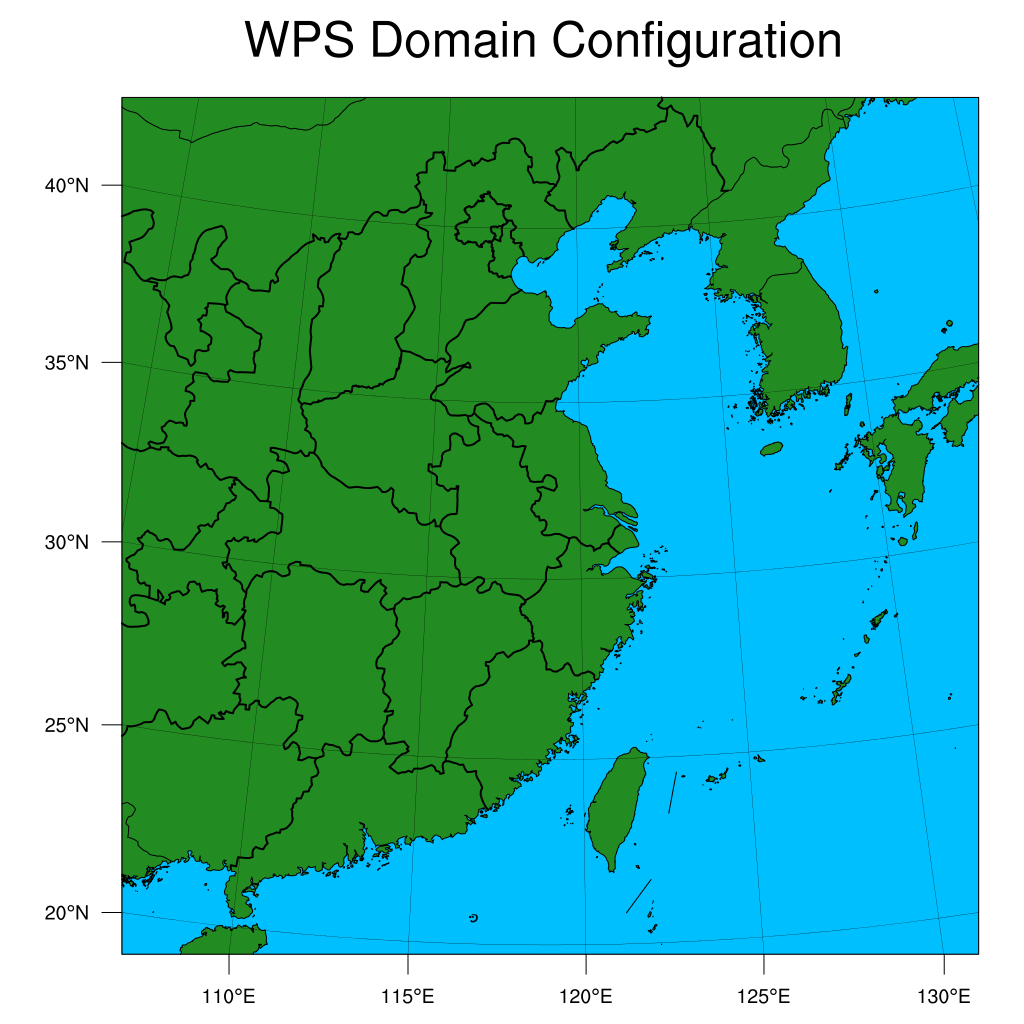
\includegraphics[trim = 15mm 5mm 5mm 24mm, clip, width=0.60\textwidth]{wps_show_dom}
    \bicaption{模拟区域}{Simulation Domain}
    \label{fig:wps_show_dom_trim}
\end{figure}

\chapter{江苏省轻污染过程数值模拟}\label{chap:evaluation}


\section{环流场形势分析}

2015年1月20日00时500hPa高空图长江中下游地区处于低压槽前,槽前受西南气流控制。21日12时槽线过境,受槽后西北气流控制。地面图上,江苏南京1月20日受低压控制,盛行风方向为低压前部偏南风控制,21日12时后受来自上游蒙古高压控制,天气条件稳定有利于污染物的累积。方向由高压前部偏北风向转为高压后部偏南风。

\begin{figure}[!htbp]
    \centering
    \begin{subfigure}[b]{0.40\textwidth}
      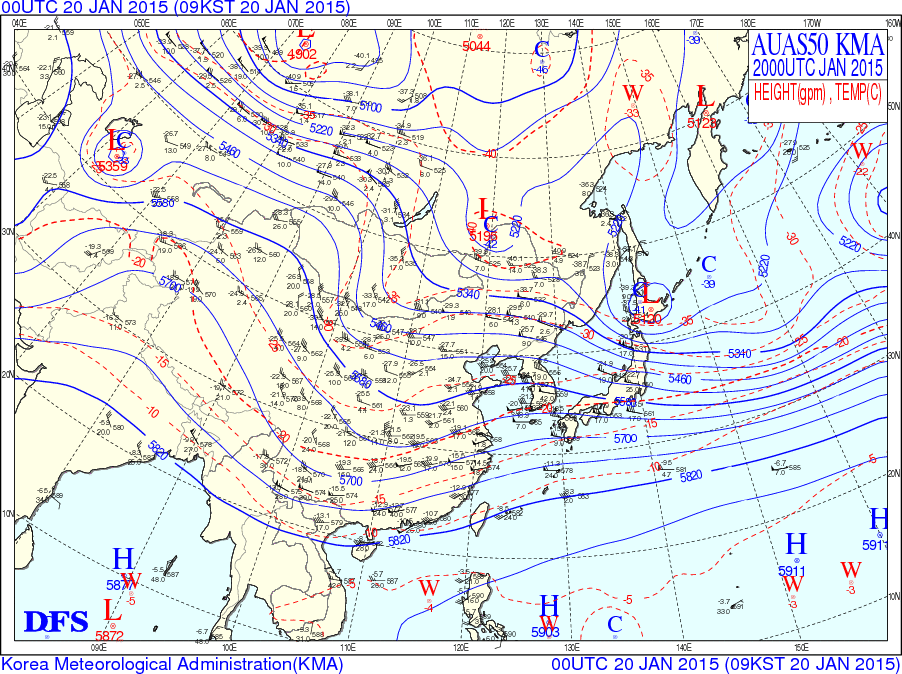
\includegraphics[width=\textwidth]{up50_2015012000}
      \caption{}
      \label{fig:up50_2015012000}
    \end{subfigure}%
    ~% add desired spacing
    \begin{subfigure}[b]{0.40\textwidth}
      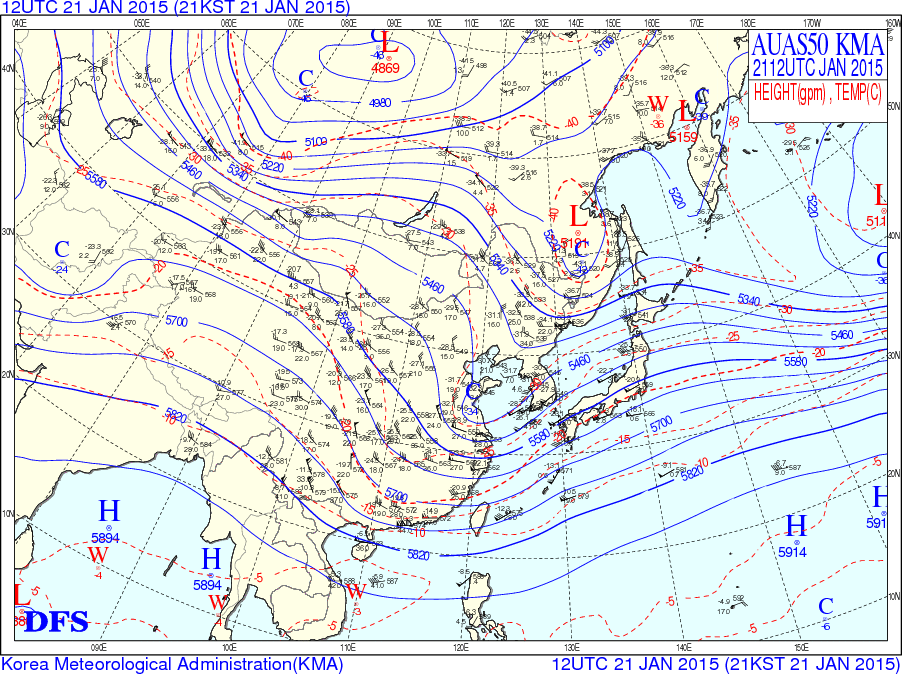
\includegraphics[width=\textwidth]{up50_2015012112}
      \caption{}
      \label{fig:up50_2015012112}
    \end{subfigure}
    \\% line break
    \begin{subfigure}[b]{0.40\textwidth}
      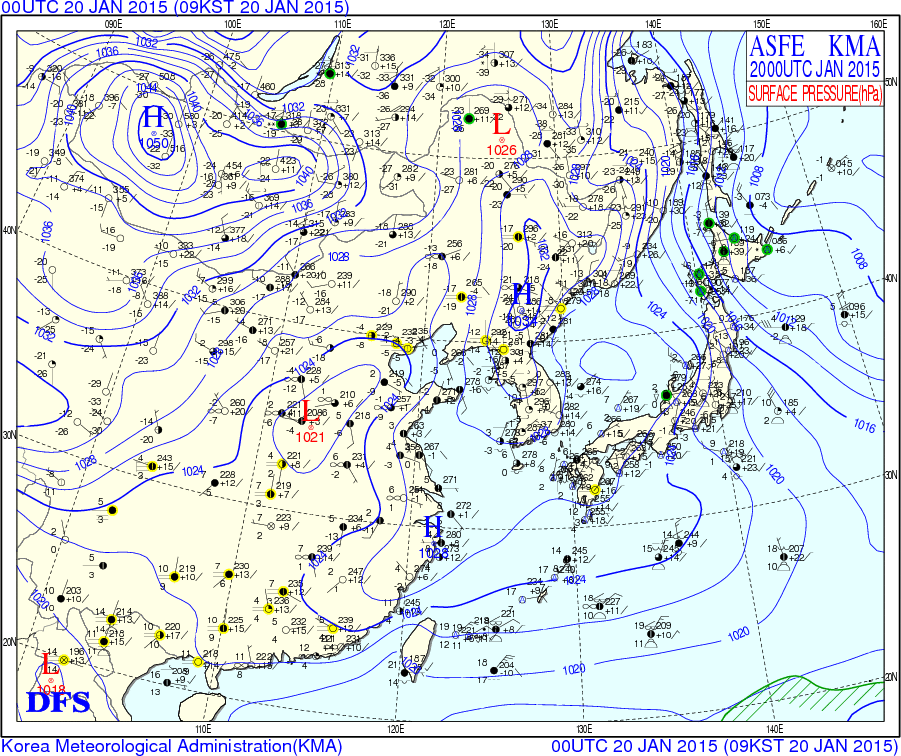
\includegraphics[width=\textwidth]{sfc3_2015012000}
      \caption{}
      \label{fig:sfc3_2015012000}
    \end{subfigure}%
    ~% add desired spacing
    \begin{subfigure}[b]{0.40\textwidth}
      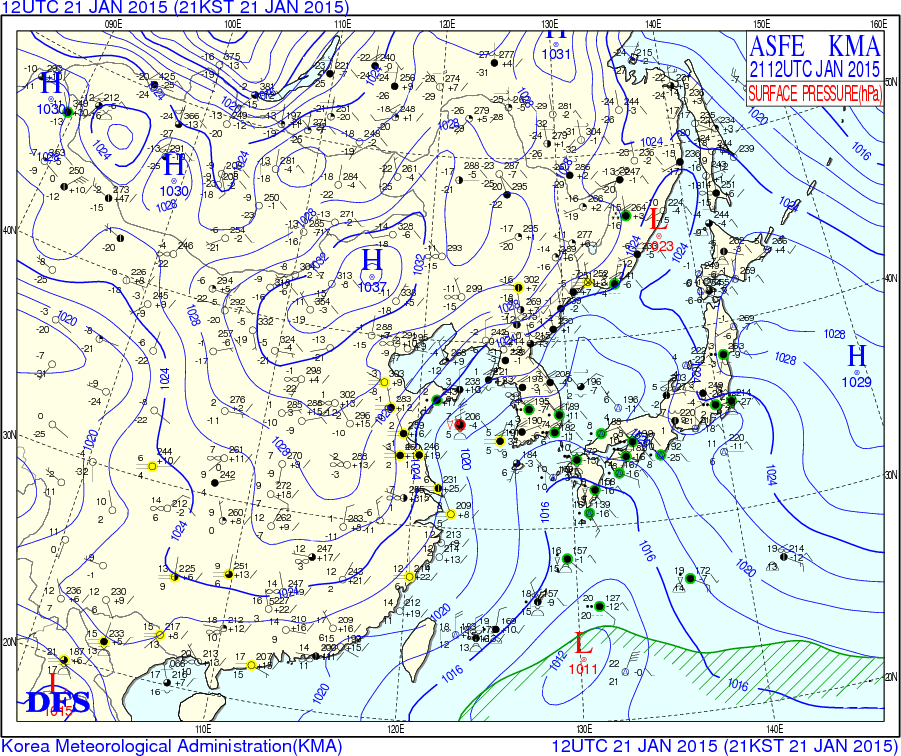
\includegraphics[width=\textwidth]{sfc3_2015012112}
      \caption{}
      \label{fig:sfc3_2015012112}
    \end{subfigure}
    \bicaption{韩国气象局天气图(a) 1月20日00时500hPa等高线图,(b) 1月21日12时500hPa等高线图,(c) 1月20日00时地面图,(d) 1月21日12时地面图。}{Korea Meteorological Administration (a) 500hPa Contour map on 00 a.m. on 20 January, (b) 500hPa Contour map on 12 a.m. on 21 January, (c) Groud map on 00 a.m. on 20 January, (d) Groud map on 12 a.m. on 21 January.}
    \label{fig:oaspl}
\end{figure}

\section{大气层结分析}

根据模拟结果选取污染过境前时刻绘制探空曲线来分析该此个例的大气层结状态,南京站在1月20日23时,探空曲线的温度露点差随高度先减少后增加,在700hPa附近存在较高湿度。大气层结存在较强垂直风切变,在一定的触发机制下有利于污染物在垂直方向的扩散,低空存在较为浅薄的逆温层且该站点的Cape能为0,层结较为稳定一定程度上有利于低层污染物堆积。

\begin{figure}[!htbp]
    \centering
    %trim option's parameter order: left bottom right top
    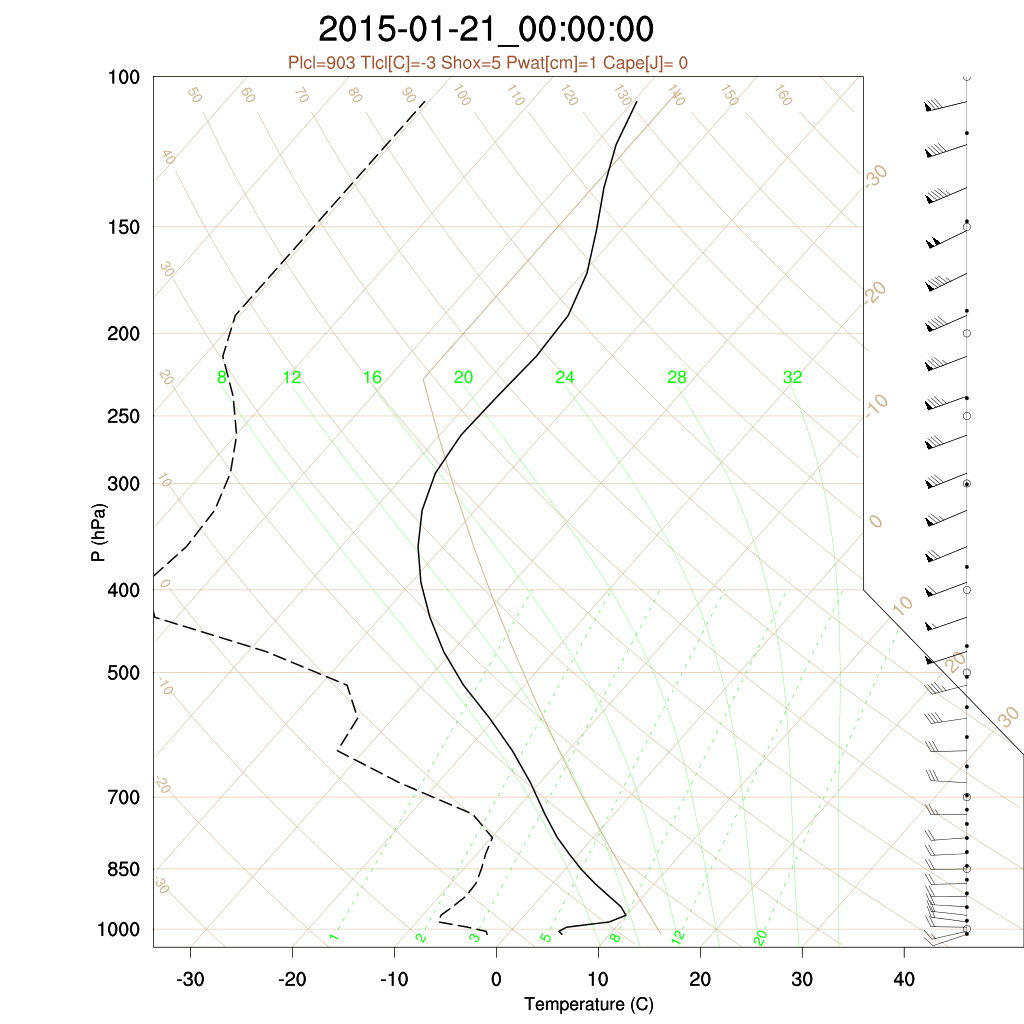
\includegraphics[trim = 5mm 0mm 0mm 0mm, clip, width=0.60\textwidth]{UW-plt_SkewT}
    \bicaption{南京站模拟的探空曲线}{Simulated sounding data curve in Nanjing station}
    \label{fig:UW-plt_SkewT_trim}
\end{figure}

\section{模拟结果评估}

通过与实况资料对比,可以发现$PM_{2.5}$,和$PM_{10}$整体浓度变化趋势一致,$PM_{10}$浓度较$PM_{2.5}$高,在22日凌晨前后模拟与观测有较大误差。CO污染物浓度较低,模拟浓度和观测浓度接近。$SO_{2}$浓度也在22日同观测有所偏差,$NO_{2}$和$O_{3}$浓度的模拟都与实况有着较高的一致性,且误差较小。

\begin{figure}[!htbp]
    \centering
    \begin{subfigure}[b]{0.40\textwidth}
      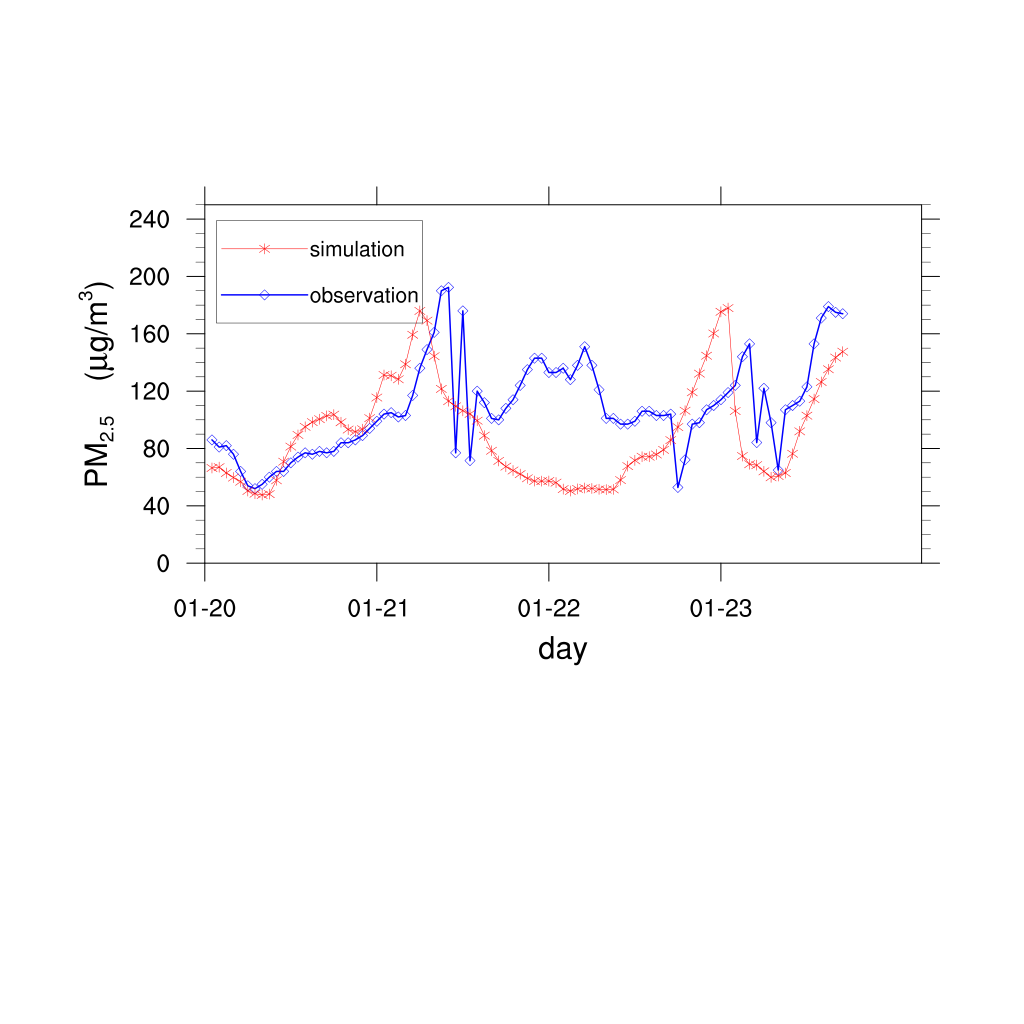
\includegraphics[trim = 20mm 120mm 30mm 50mm, clip, width=\textwidth]{plot-obe-sim-pm25}
      \caption{}
      \label{fig:plot-obe-sim-pm25}
    \end{subfigure}%
    ~% add desired spacing
    \begin{subfigure}[b]{0.40\textwidth}
      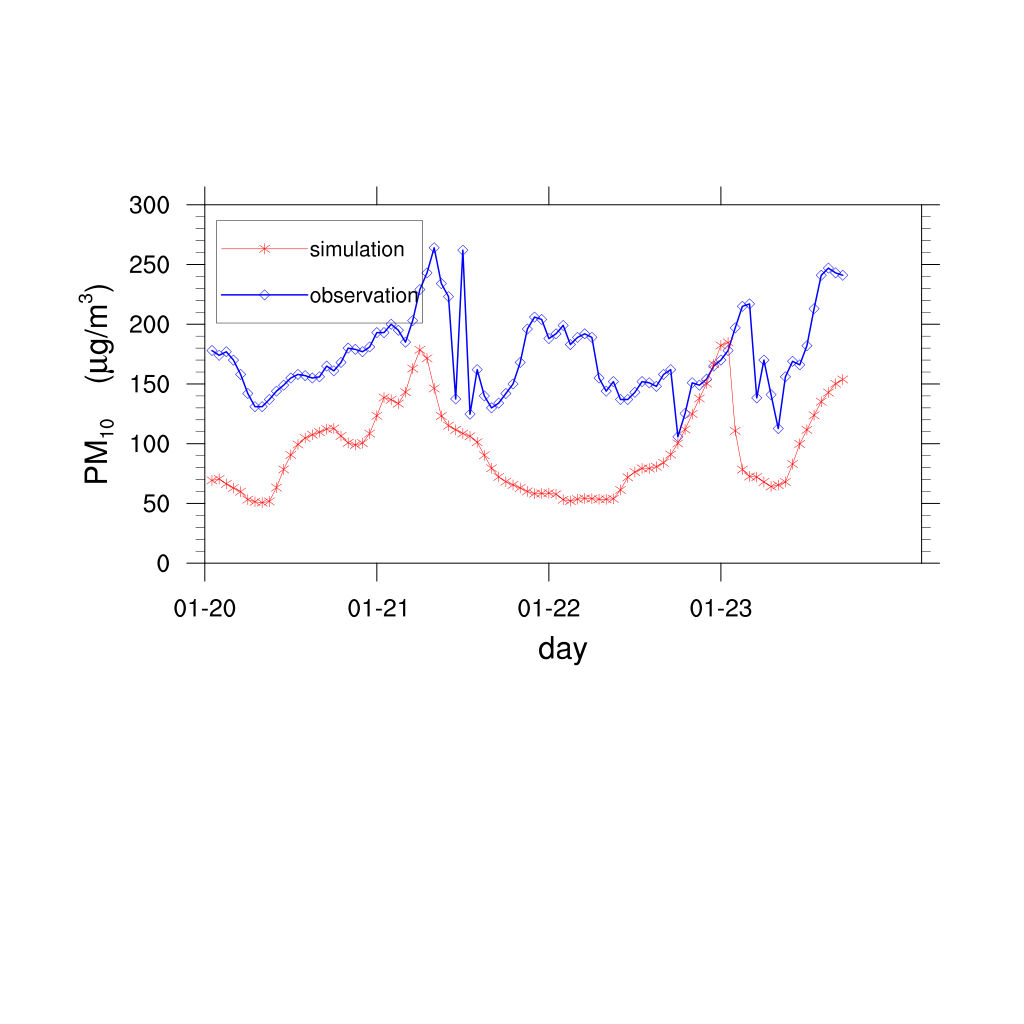
\includegraphics[trim = 20mm 120mm 30mm 50mm, clip, width=\textwidth]{plot-obe-sim-pm10}
      \caption{}
      \label{fig:plot-obe-sim-pm10}
    \end{subfigure}
    \\% line break
    \begin{subfigure}[b]{0.40\textwidth}
      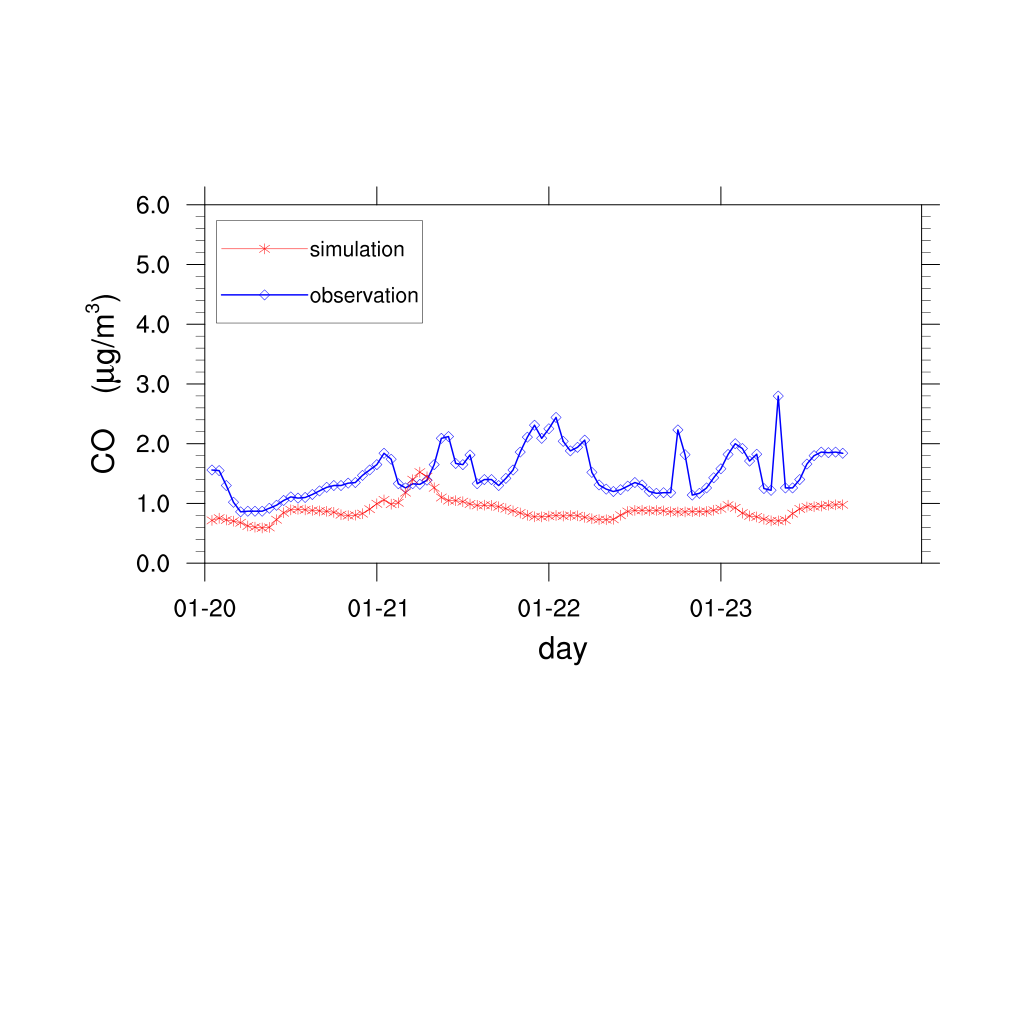
\includegraphics[trim = 20mm 120mm 30mm 50mm, clip, width=\textwidth]{plot-obe-sim-co}
      \caption{}
      \label{fig:plot-obe-sim-co}
    \end{subfigure}%
    ~% add desired spacing
    \begin{subfigure}[b]{0.40\textwidth}
      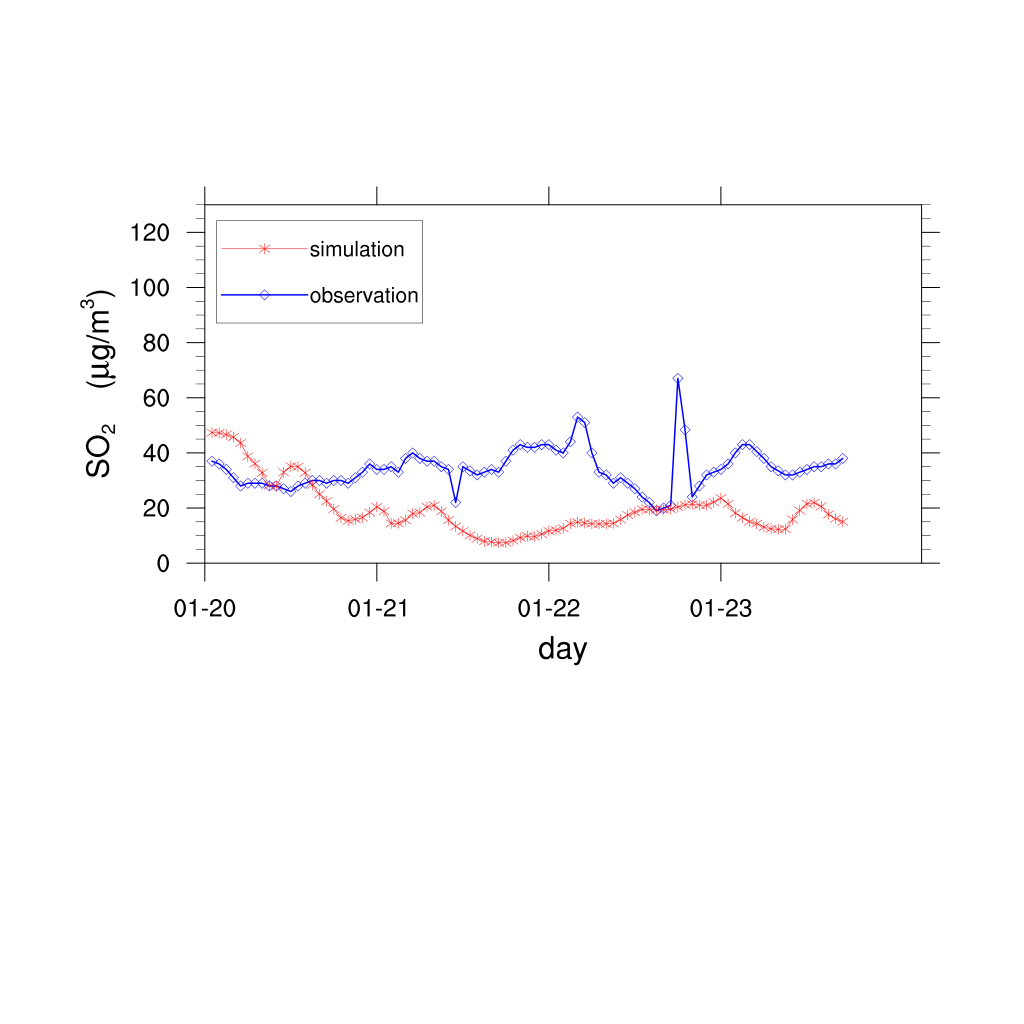
\includegraphics[trim = 20mm 120mm 30mm 50mm, clip, width=\textwidth]{plot-obe-sim-so2}
      \caption{}
      \label{fig:plot-obe-sim-so2}
    \end{subfigure}
    \begin{subfigure}[b]{0.40\textwidth}
      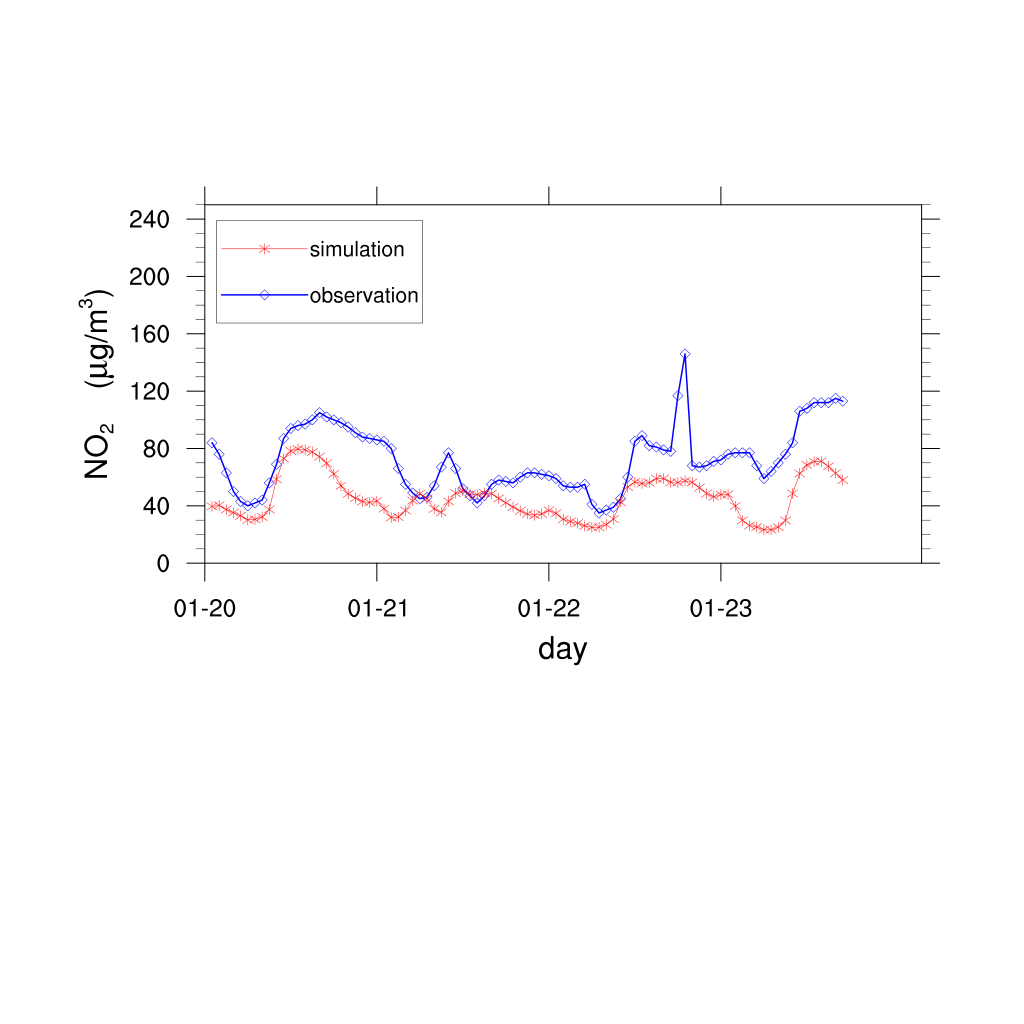
\includegraphics[trim = 20mm 120mm 30mm 50mm, clip, width=\textwidth]{plot-obe-sim-no2}
      \caption{}
      \label{fig:plot-obe-sim-no2}
    \end{subfigure}
    \begin{subfigure}[b]{0.40\textwidth}
      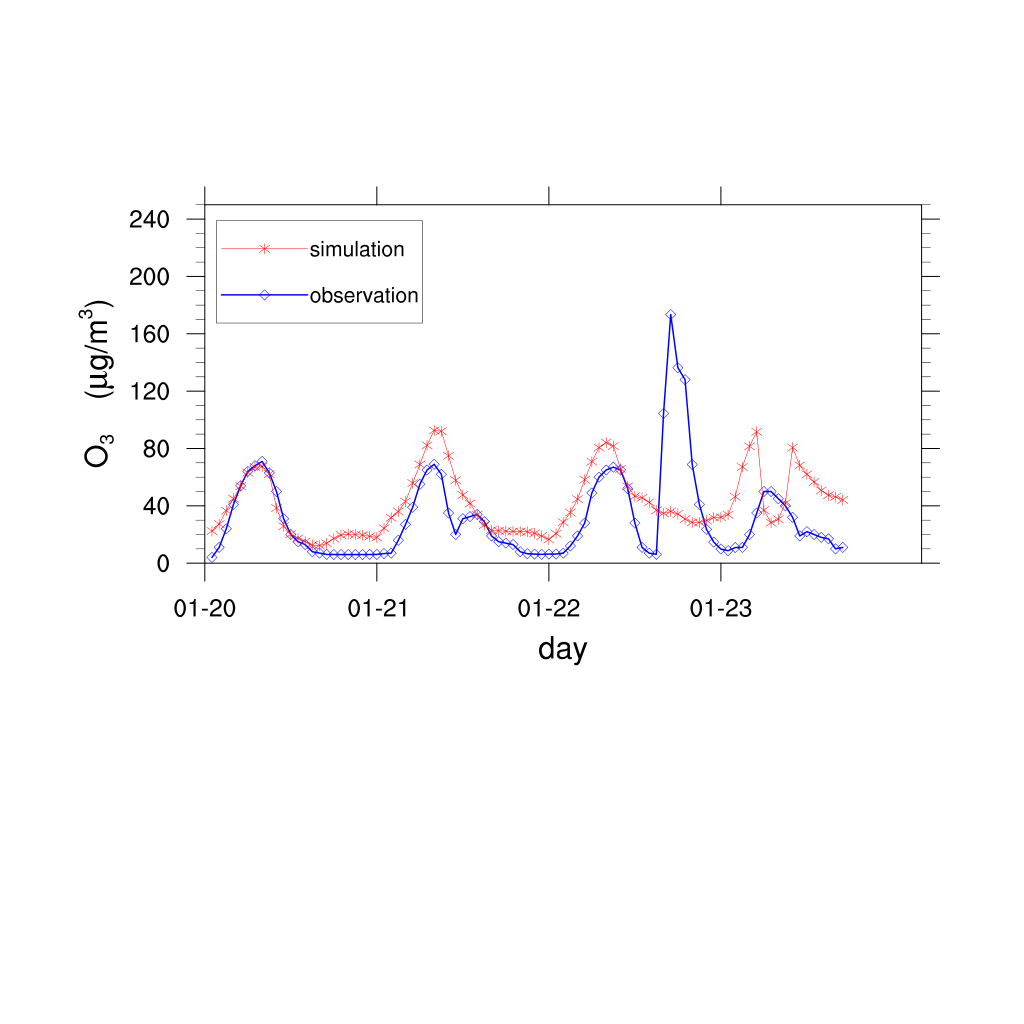
\includegraphics[trim = 20mm 120mm 30mm 50mm, clip, width=\textwidth]{plot-obe-sim-o3}
      \caption{}
      \label{fig:plot-obe-sim-o3}
    \end{subfigure}

		\bicaption{模拟与观测的污染物浓度对比 (a) $PM_{2.5}$浓度,(b) $PM_{10}$浓度,(c) CO浓度,(d) $SO_{2}$浓度,(e) $NO_{2}$浓度,(f) $O_{3}$浓度。}{(a) The concentration of $PM_{2.5}$, (b) The concentration of $PM_{10}$, (c) The concentration of CO, (d) The concentration of $SO_{2}$, (e) The concentration of $NO_{2}$, (f) The concentration of $O_{3}$.}

    \label{fig:oaspl}
\end{figure}

\section{边界层高度}

不同边界层参数化方案计算边界层高度的方法不一,MRF、YSU方案均通过临界理查逊数法确定边界层高度,通过统一算法计算区域平均边界层高度,其中g为重力加速度,$\theta$为位温,z为高度,u,v为风速的纬向和经向分量,通过计算某层的总体理查逊数大于或等于临界理查逊数即0.25时,通过线性插值,将此高度确定为边界层高度。总体理查逊数的公式为:

\begin{equation}
    \adddotsbeforeeqnnum%
		R_{b} = \frac{\frac{g}{\overline{\theta}}\frac{\Delta \overline{\theta}}{\Delta z}}{(\frac{\Delta \overline{u}}{\Delta z})^2 + (\frac{\Delta \overline{v}}{\Delta z})^2}
\end{equation}

YSU方案定义边界层高度h为逆温层中湍流通量最低值所在高度,即:

\begin{equation}
    \adddotsbeforeeqnnum%
		h = Rib_{cr} \frac{\theta_{va}|U(h)|^{2}}{g[\theta_{v}(h)-\theta_{s}]}
\end{equation}

选取江苏省区域来计算平均边界层高度


\begin{figure}[!htbp]
    \centering
    %trim option's parameter order: left bottom right top
    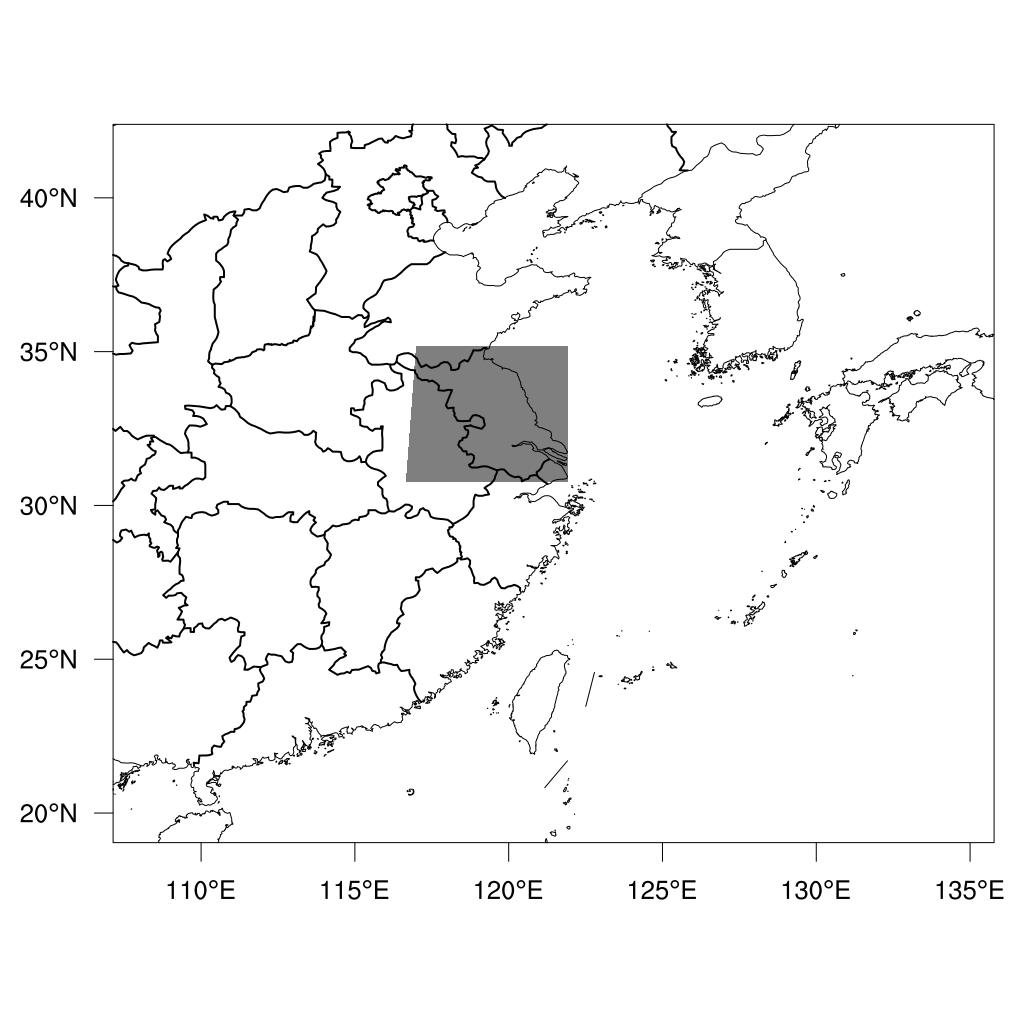
\includegraphics[trim = 2mm 10mm 0mm 10mm, clip, width=0.60\textwidth]{poly_ex}
    \bicaption{平均边界层高度对应区域}{The region corresponding to the mean boundary layer height}
		\label{fig:poly_ex}
\end{figure}

\section{边界层与污染物浓度关系}

随着白天温度的上升,热力对流作用占据对流的主导地位,大多数污染物都在对流扩散稀释的作用下,随着边界层的高度增加,其浓度均有所下降,呈现负相关。对流层臭氧却与边界层高度呈现正相关,主要原因是由于,臭氧的生成需要光照和热量,对流边界层的高度白天大于夜间,也受热力影响,因而在午后臭氧的浓度均达到峰值,同时可以从图中可以发现臭氧的峰值变化相交边界层高度更具有周期性,由此臭氧对日变化更具敏感性。

\begin{figure}[!htbp]
    \centering
    \begin{subfigure}[b]{0.40\textwidth}
      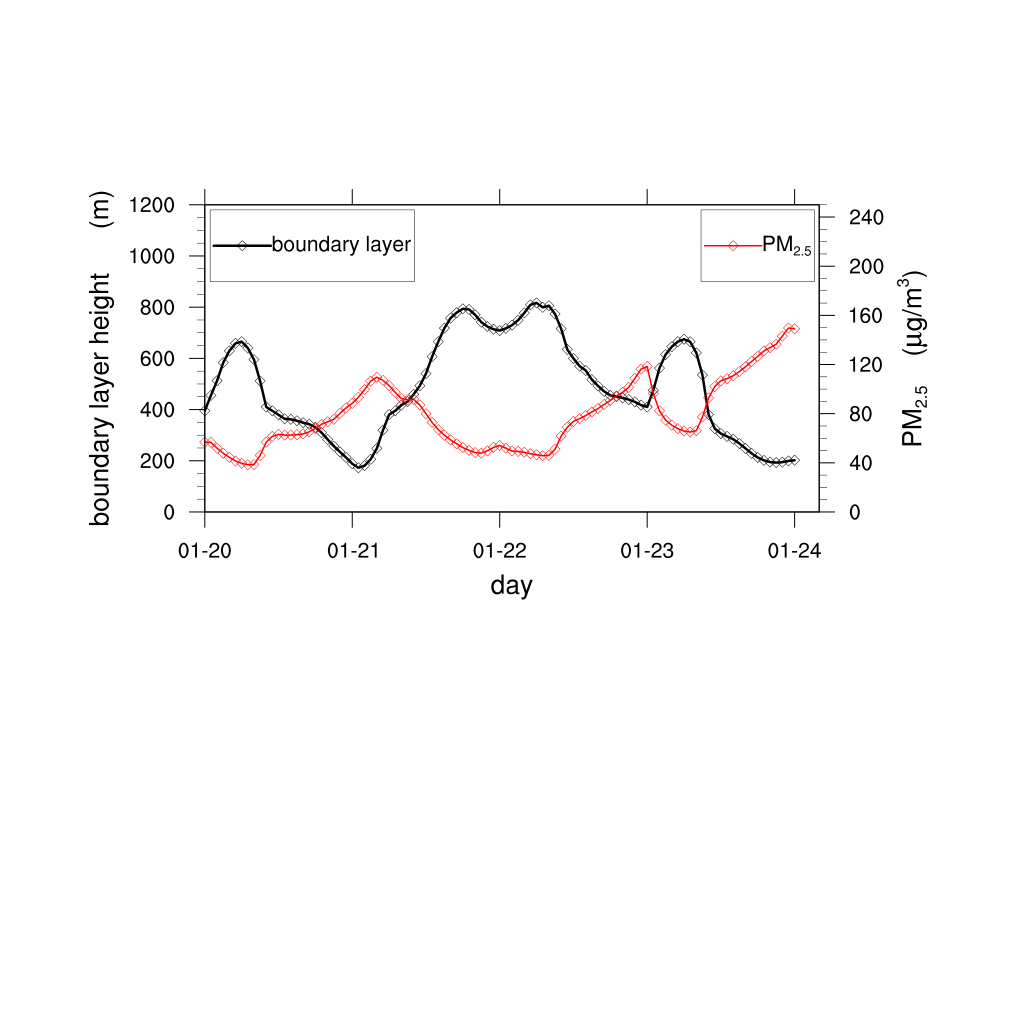
\includegraphics[trim = 20mm 120mm 30mm 50mm, clip, width=\textwidth]{bjl_pm25}
      \caption{}
      \label{fig:bjl_pm25}
    \end{subfigure}%
    ~% add desired spacing
    \begin{subfigure}[b]{0.40\textwidth}
      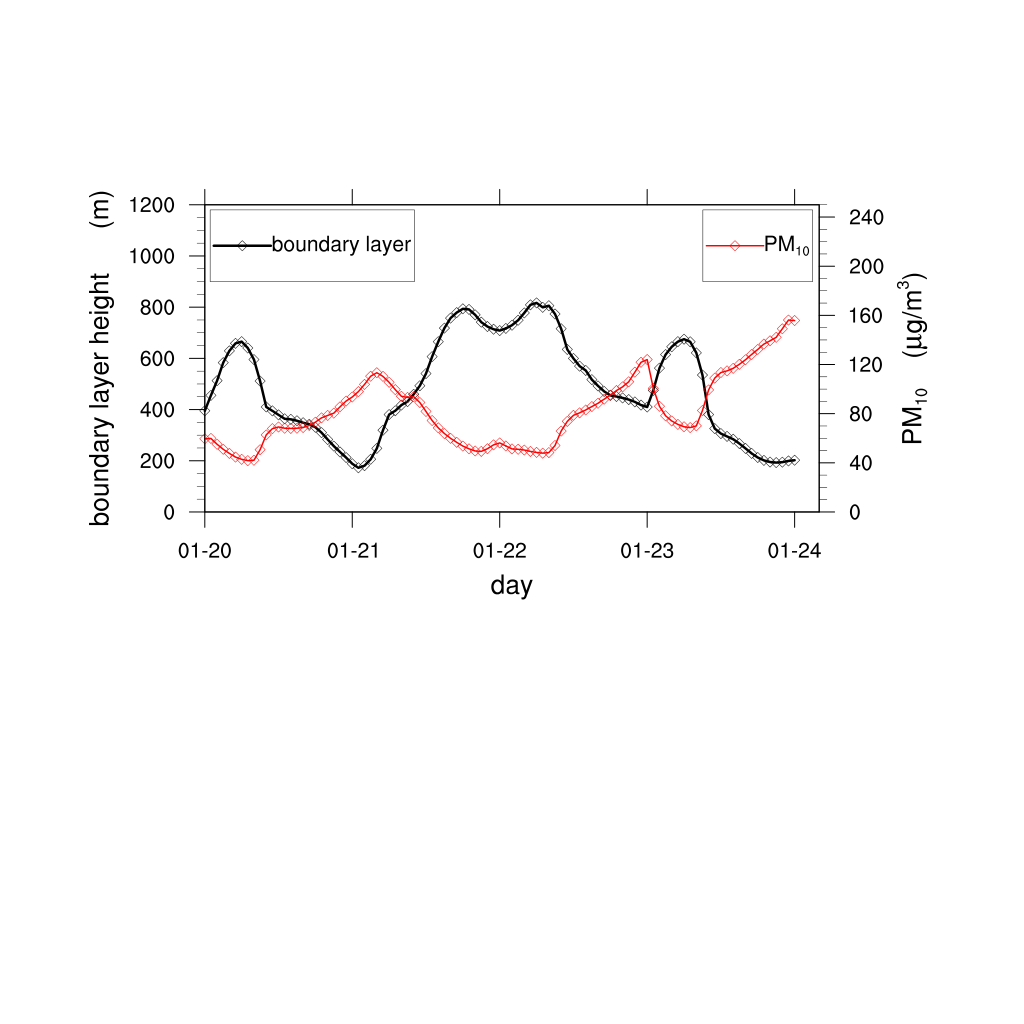
\includegraphics[trim = 20mm 120mm 30mm 50mm, clip, width=\textwidth]{bjl_pm10}
      \caption{}
			\label{fig:bjl_pm10}
    \end{subfigure}
    \\% line break
    \begin{subfigure}[b]{0.40\textwidth}
      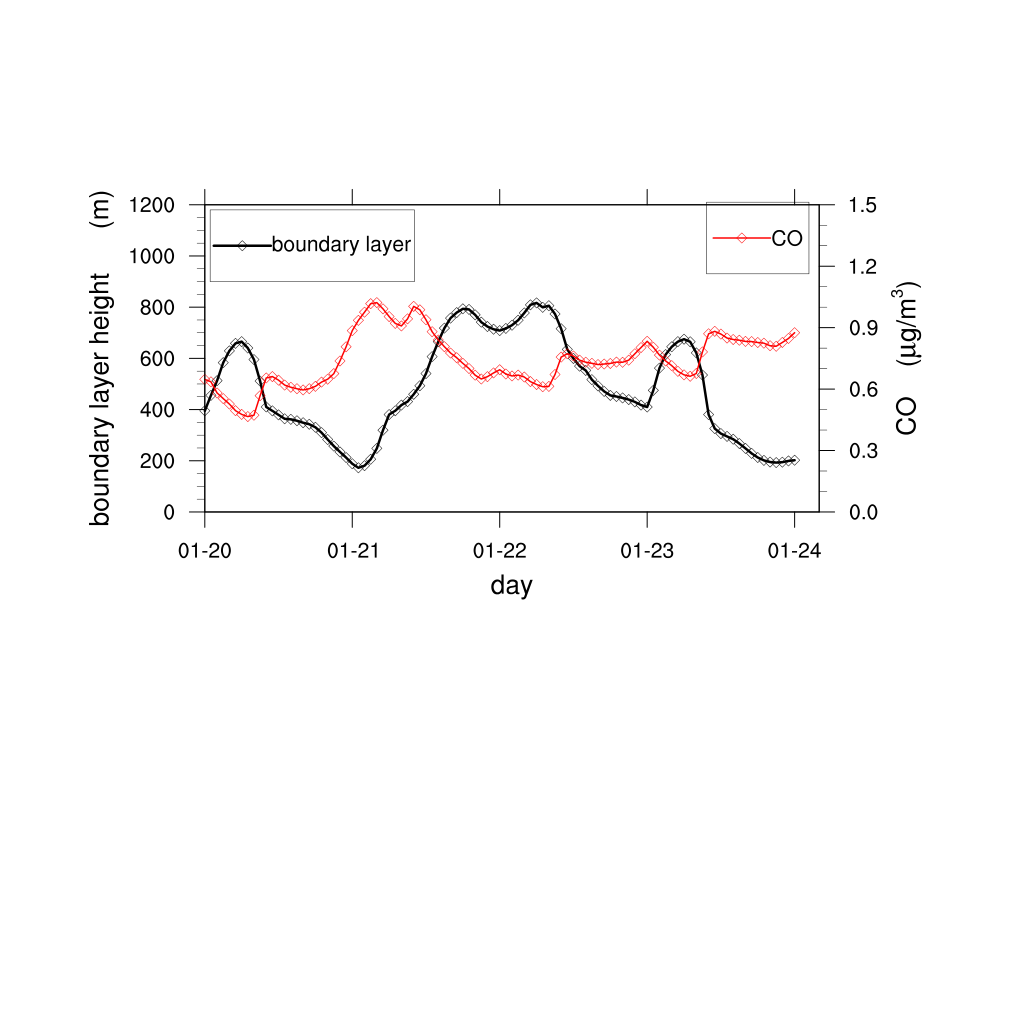
\includegraphics[trim = 20mm 120mm 30mm 50mm, clip, width=\textwidth]{bjl_co}
      \caption{}
			\label{fig:bjl_co}
    \end{subfigure}%
    ~% add desired spacing
    \begin{subfigure}[b]{0.40\textwidth}
      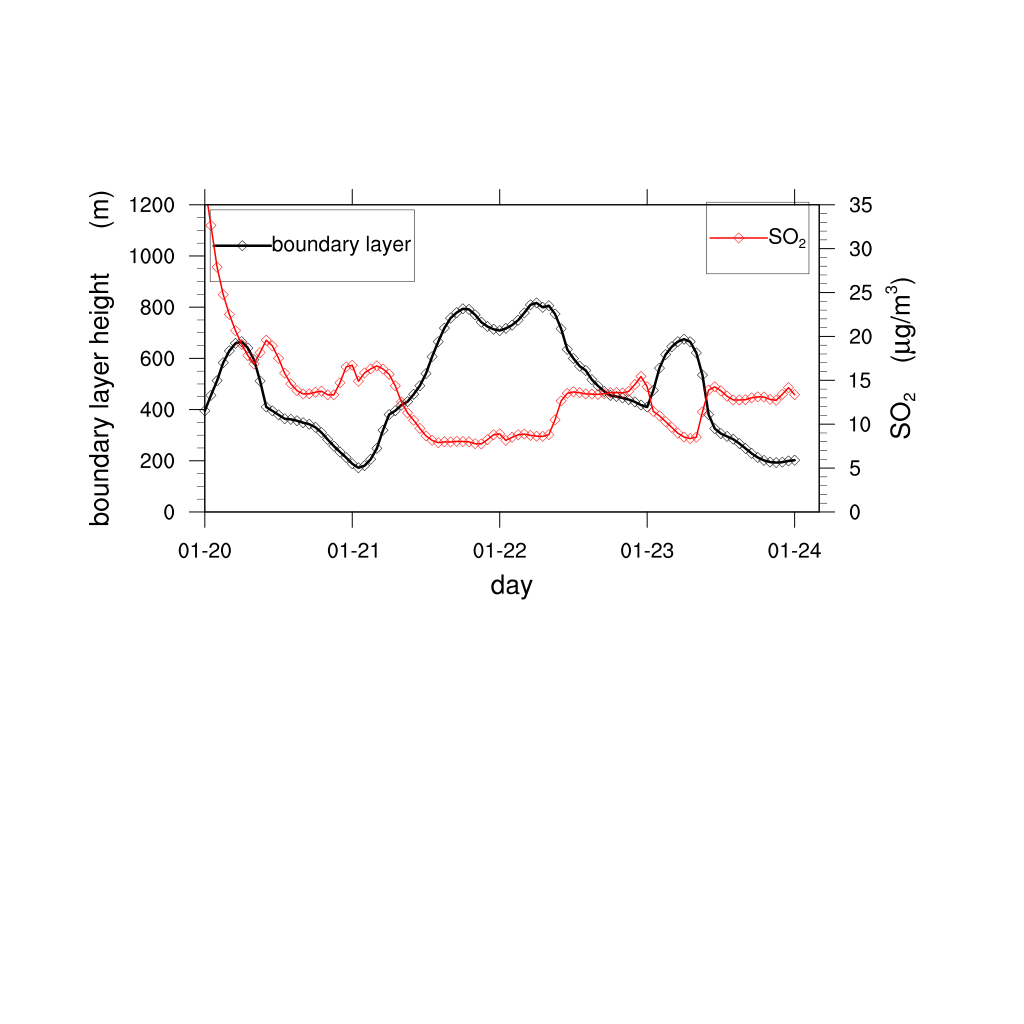
\includegraphics[trim = 20mm 120mm 30mm 50mm, clip, width=\textwidth]{bjl_so2}
      \caption{}
			\label{fig:bjl_so2}
    \end{subfigure}
    \begin{subfigure}[b]{0.40\textwidth}
      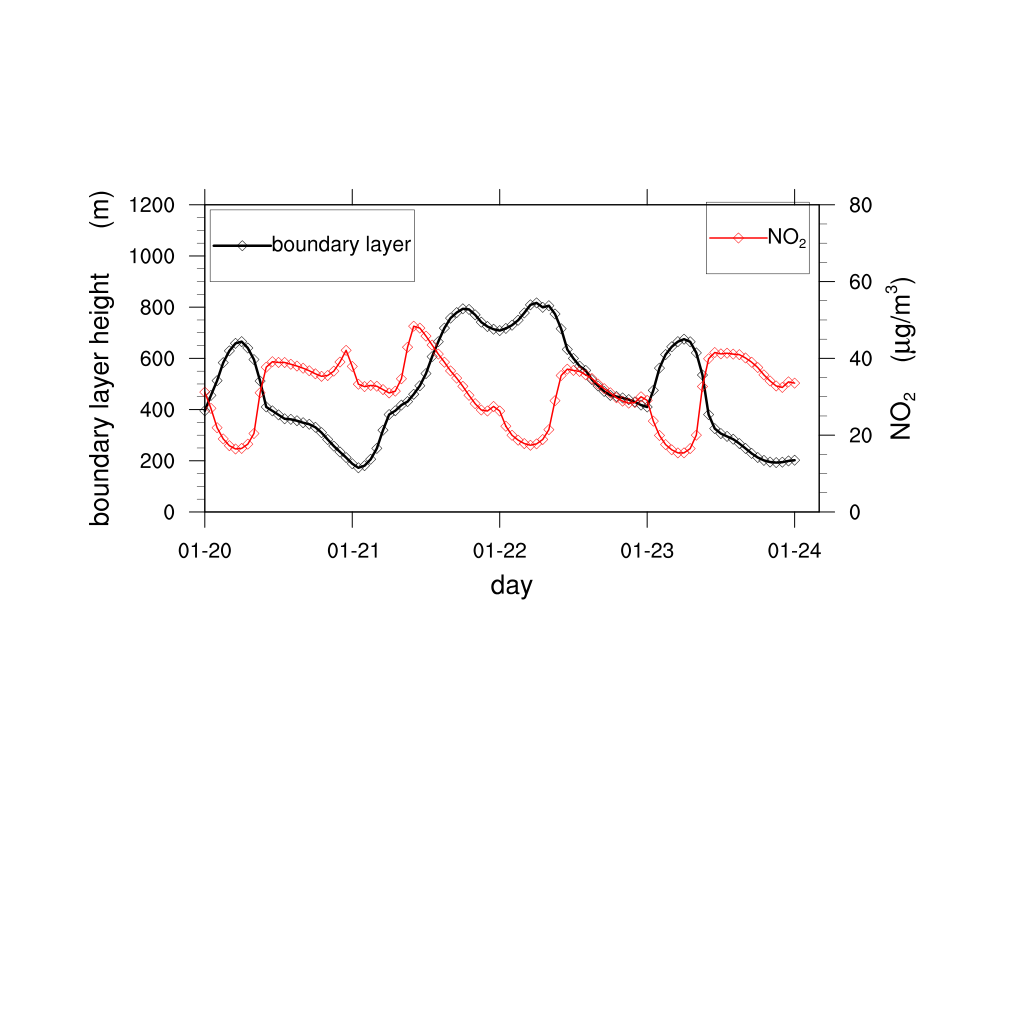
\includegraphics[trim = 20mm 120mm 30mm 50mm, clip, width=\textwidth]{bjl_no2}
      \caption{}
			\label{fig:bjl_no2}
    \end{subfigure}
    \begin{subfigure}[b]{0.40\textwidth}
      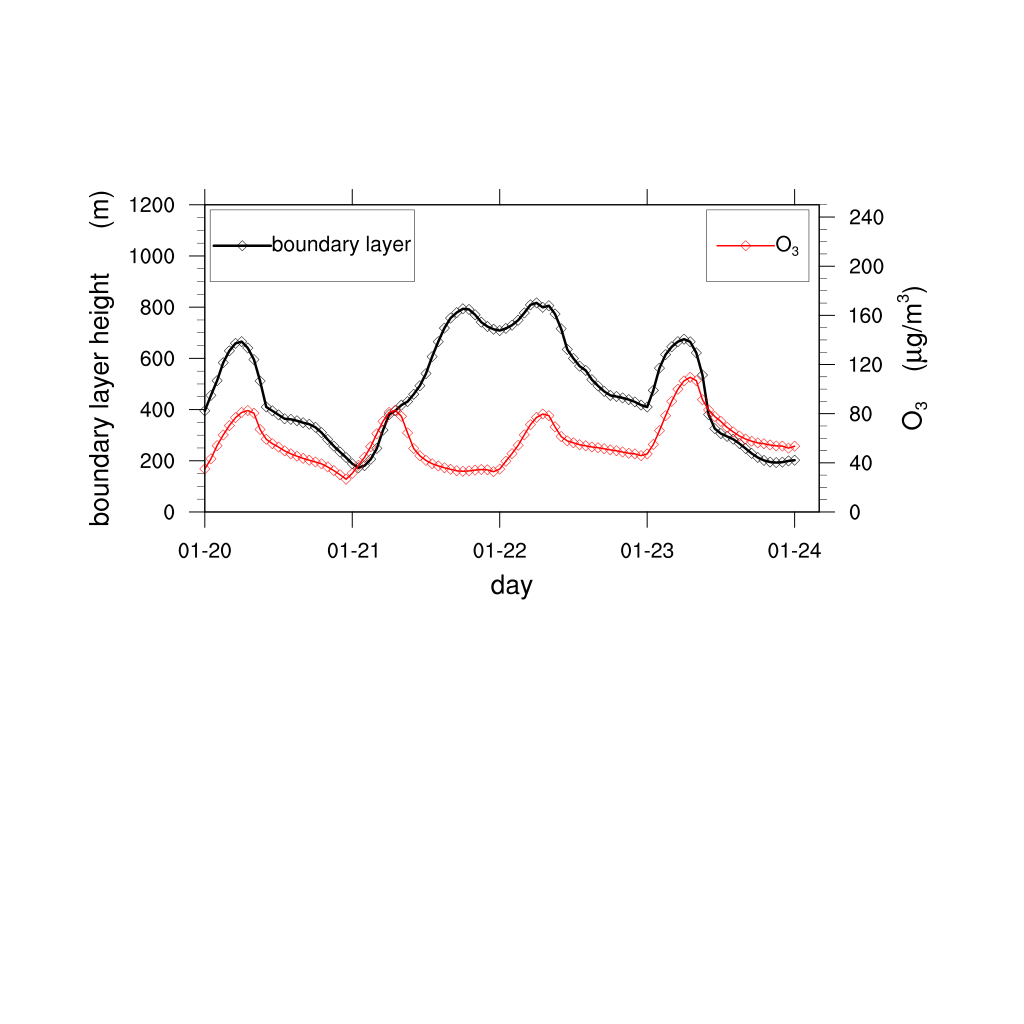
\includegraphics[trim = 20mm 120mm 30mm 50mm, clip, width=\textwidth]{bjl_o3}
      \caption{}
			\label{fig:bjl_o3}
    \end{subfigure}
		\bicaption{边界层高度与污染物浓度对比 (a) $PM_{2.5}$浓度,(b) $PM_{10}$浓度,(c) CO浓度, (d) $SO_{2}$浓度, (e) $NO_{2}$浓度,(f) $O_{3}$浓度。}{Comparison between Boundary layer height and pollution concentration (a) The concentration of $PM_{2.5}$, (b) The concentration of $PM_{10}$, (c) The concentration of CO, (d) The concentration of $SO_{2}$, (e) The concentration of $NO_{2}$, (f) The concentration of $O_{3}$.}
		\label{fig:oaspl}
\end{figure}


\section{$PM_{2.5}$水平分布特征}

根据$PM_{2.5}$浓度水平分布可以分析得污染物整体跟随天气配置槽线位置移动,$PM_{2.5}$污染物源自河南河北地区,21日07时跟随风场移动扩散迁移至江苏地区且浓度达到极大值,随后污染物东移入海减弱消散。

\begin{figure}[!htbp]
	\centering
	\begin{subfigure}[b]{0.40\textwidth}
		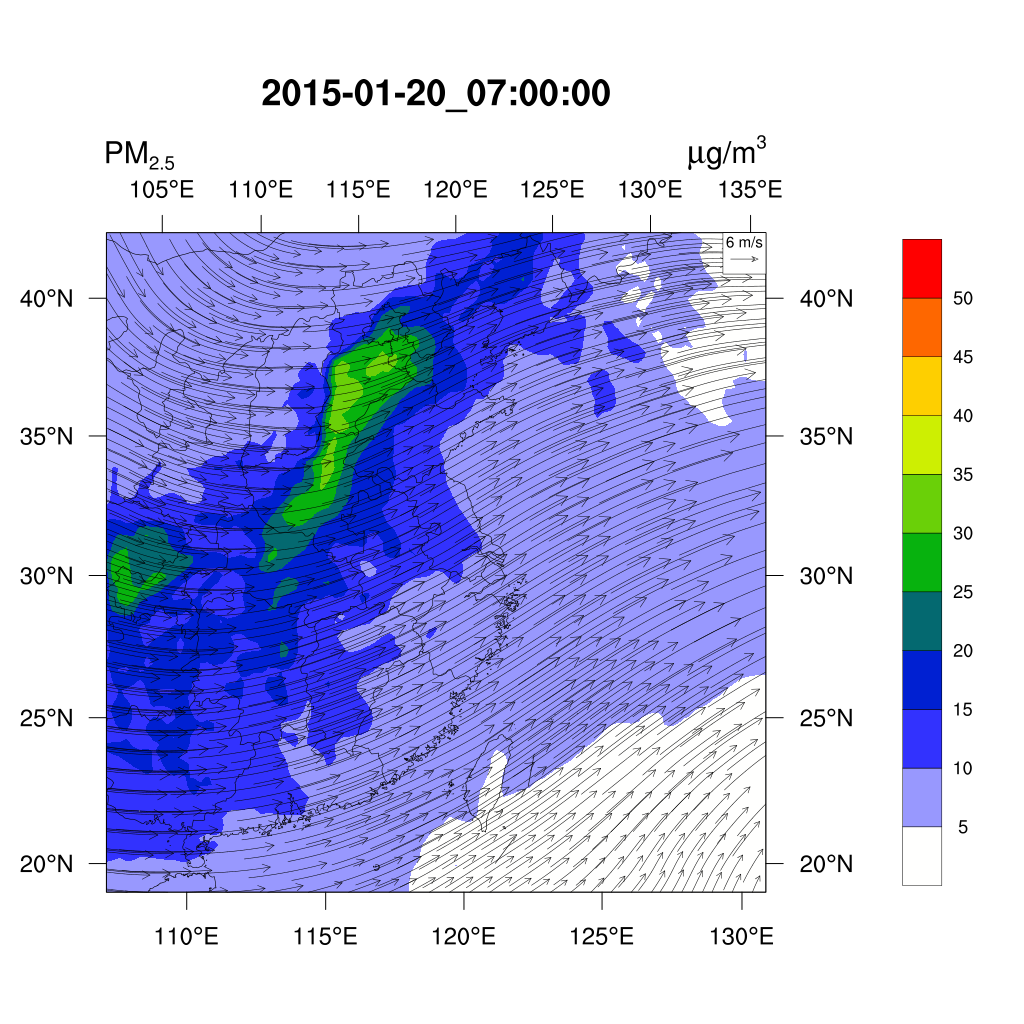
\includegraphics[width=\textwidth]{wrf_pm25_vec_000008}
		\caption{}
		\label{fig:wrf_pm25_vec_000008}
	\end{subfigure}%
	~% add desired spacing
	\begin{subfigure}[b]{0.40\textwidth}
		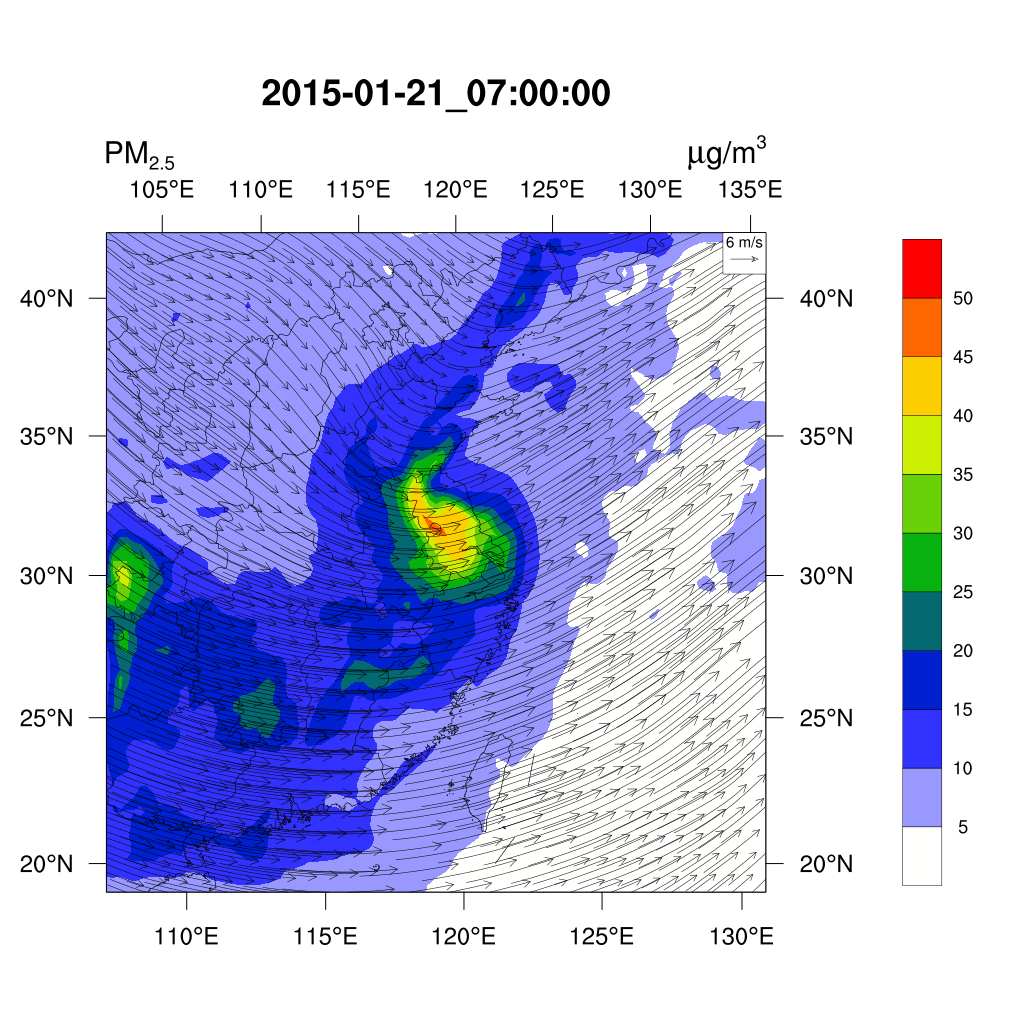
\includegraphics[width=\textwidth]{wrf_pm25_vec_000032}
		\caption{}
		\label{fig:wrf_pm25_vec_000032}
	\end{subfigure}
	\\% line break
	\begin{subfigure}[b]{0.40\textwidth}
		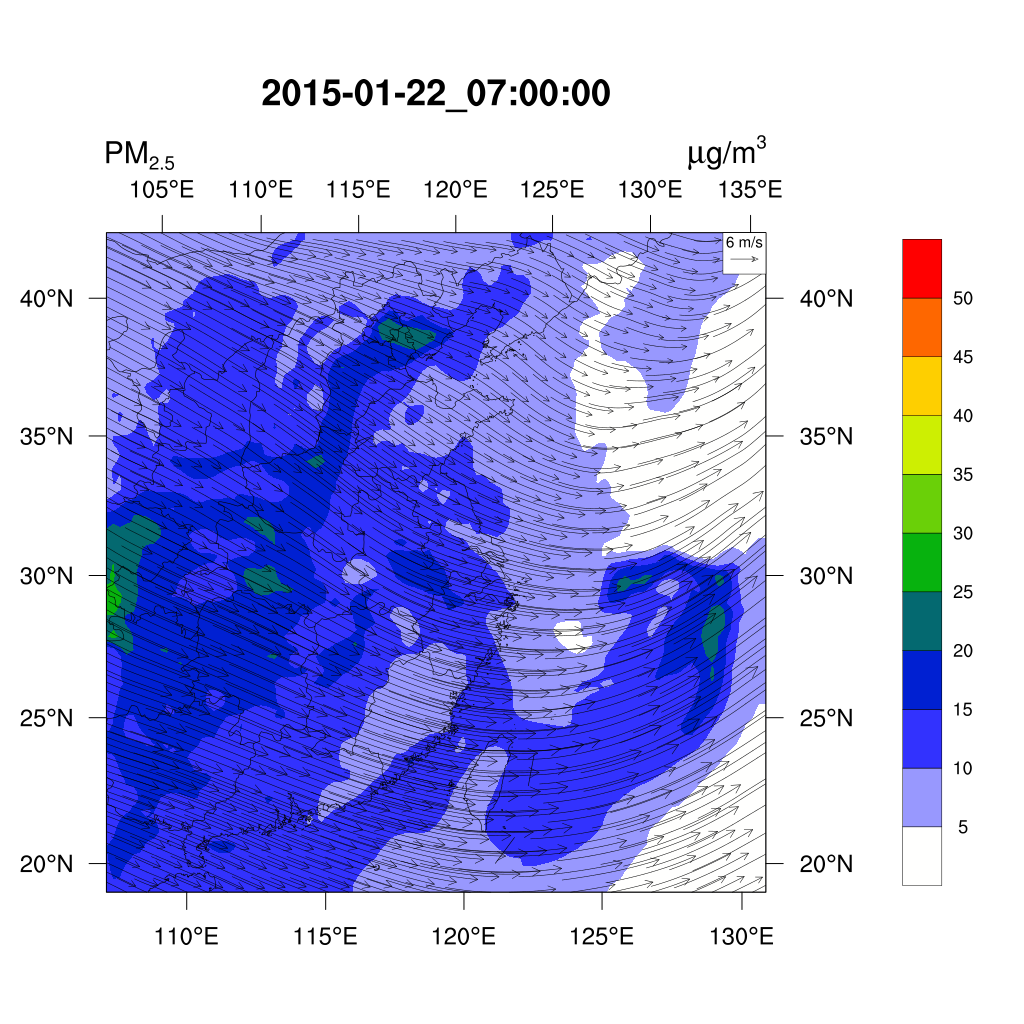
\includegraphics[width=\textwidth]{wrf_pm25_vec_000056}
		\caption{}
		\label{fig:wrf_pm25_vec_000032}
	\end{subfigure}
	~% add desired spacing
	\begin{subfigure}[b]{0.40\textwidth}
		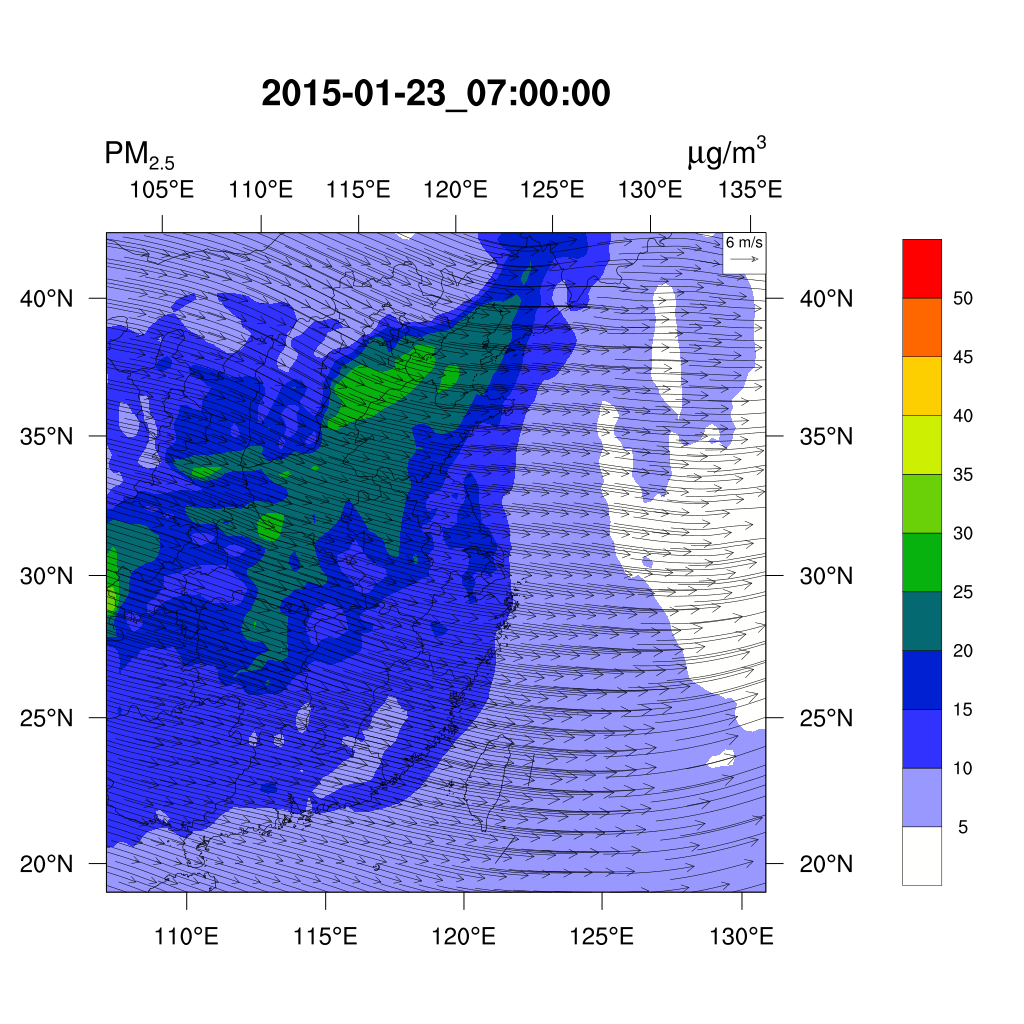
\includegraphics[width=\textwidth]{wrf_pm25_vec_000080}
		\caption{}
		\label{fig:wrf_pm25_vec_000032}
	\end{subfigure}
	\bicaption{地面$PM_{2.5}$浓度叠加风场图(a) 1月20日07时500,(b) 1月21日07时,(c) 1月21日07时,(d) 1月22日07时。}{Surface $PM_{2.5}$ concentration superimposed wind field map (a) 07 a.m. on 20 January, (b) 07 a.m. on 21 January, (c) 07 a.m. on 22 January, (d) 07 a.m. on 23 January.}
	\label{fig:oaspl}
\end{figure}

\section{$PM_{2.5}$垂直分布特征}

沿着经度线$118.907^\circE$做从$31.0^\circN$至$34.0^\circN$的剖面,从剖面图分析可发现20日00是高空收槽前西南气流,同地面低压前部偏南气流控制,整体污染物层结分布明显,随着高度污染物浓度逐渐减小,随着太阳升起日照作用下污染物逐渐向上扩散使得高层污染物浓度增加。18时受到风场带来的西北方向的近地面$PM_{2.5}$污染物使得低层污染物浓度增高,原本污染高值区被迫抬升,形成对流热泡状,且高低层风向相反,存在大的垂直风切变,动力不稳定有利于污染物向高空垂直方向的扩散。21日00时槽线过境,污染物扩散至3km以上,06时受到槽后西北气流和地面高压前部的偏北气流,使得整个层结收到偏北风影响,有利于污染累计。最终污染物随西南风向西向南移动,离开剖面区域。

\begin{figure}[!htbp]
	\centering
	\begin{subfigure}[b]{0.35\textwidth}
		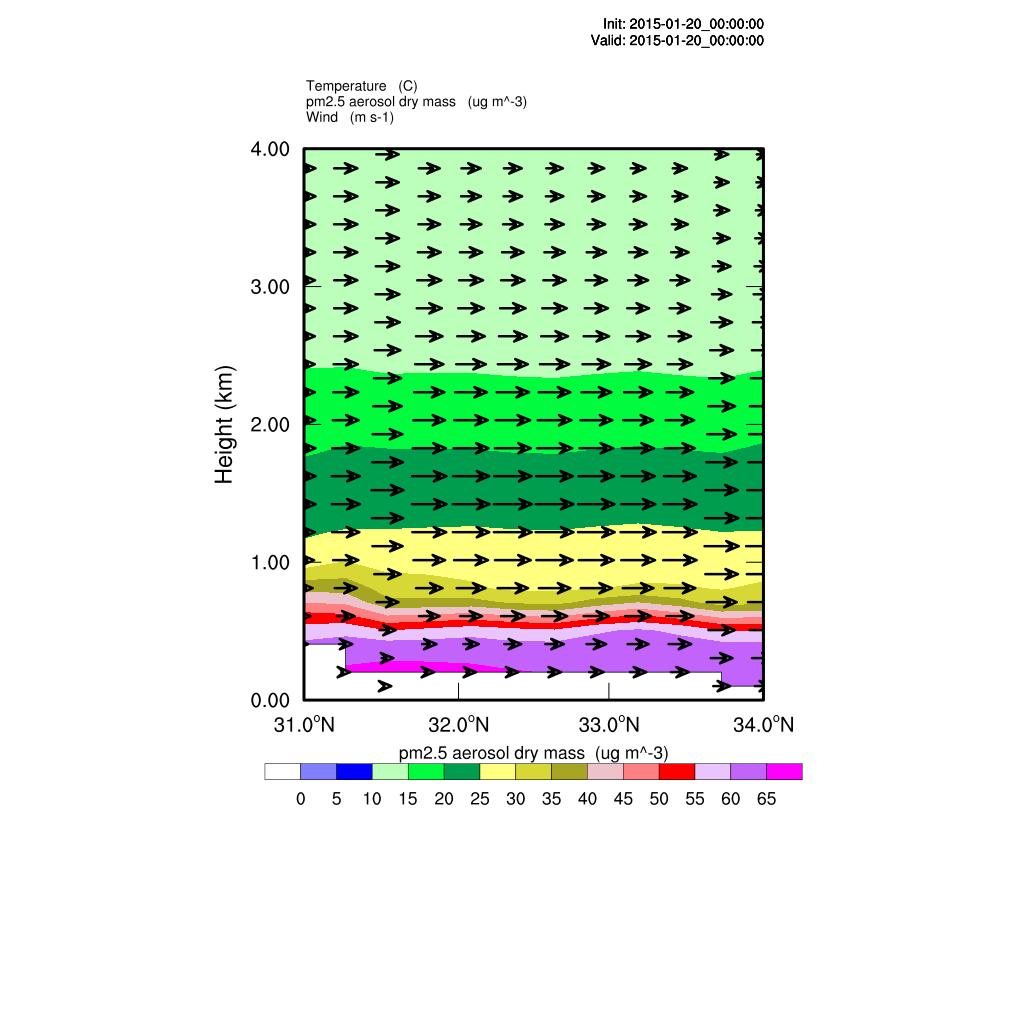
\includegraphics[width=\textwidth]{pm25_01}
		\caption{}
		\label{fig:pm25_01}
	\end{subfigure}%
	~% add desired spacing
	\begin{subfigure}[b]{0.35\textwidth}
		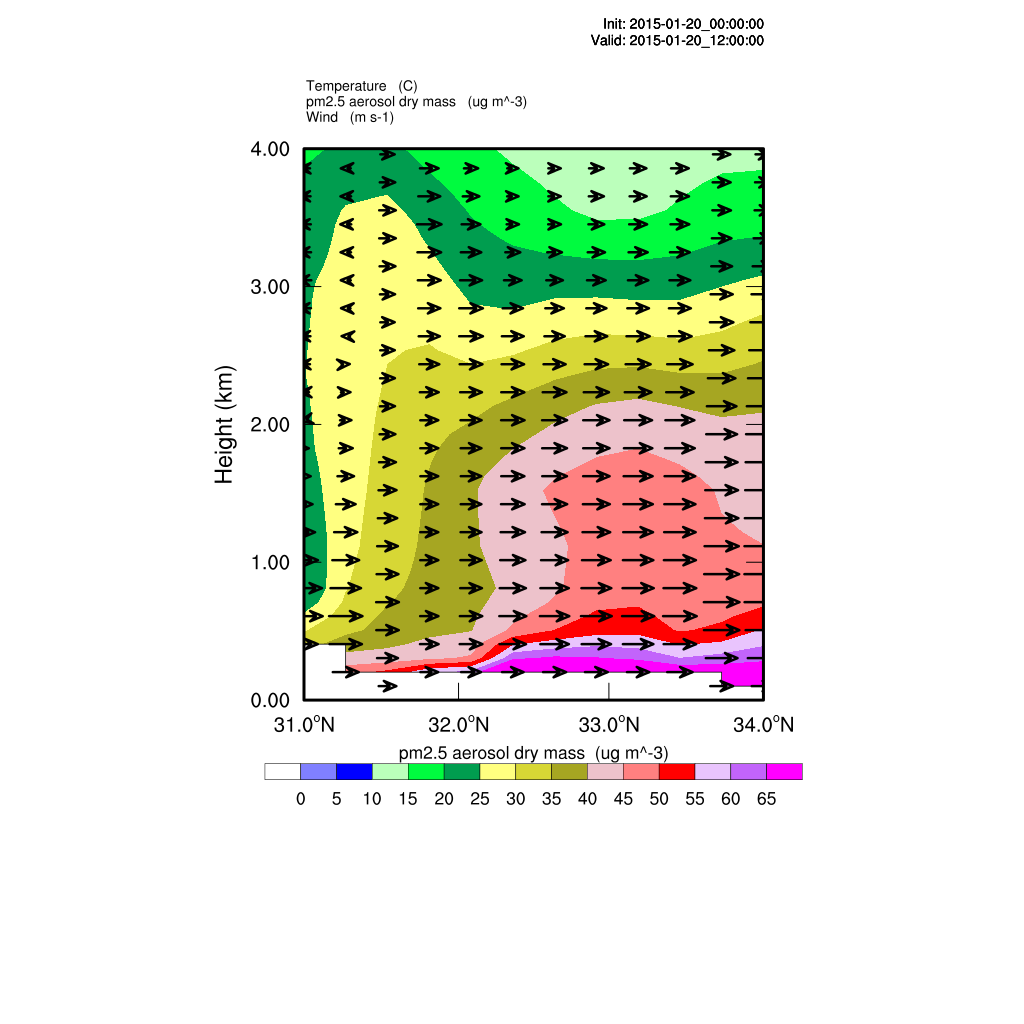
\includegraphics[width=\textwidth]{pm25_13}
		\caption{}
		\label{fig:pm25_13}
	\end{subfigure}%
	\begin{subfigure}[b]{0.35\textwidth}
		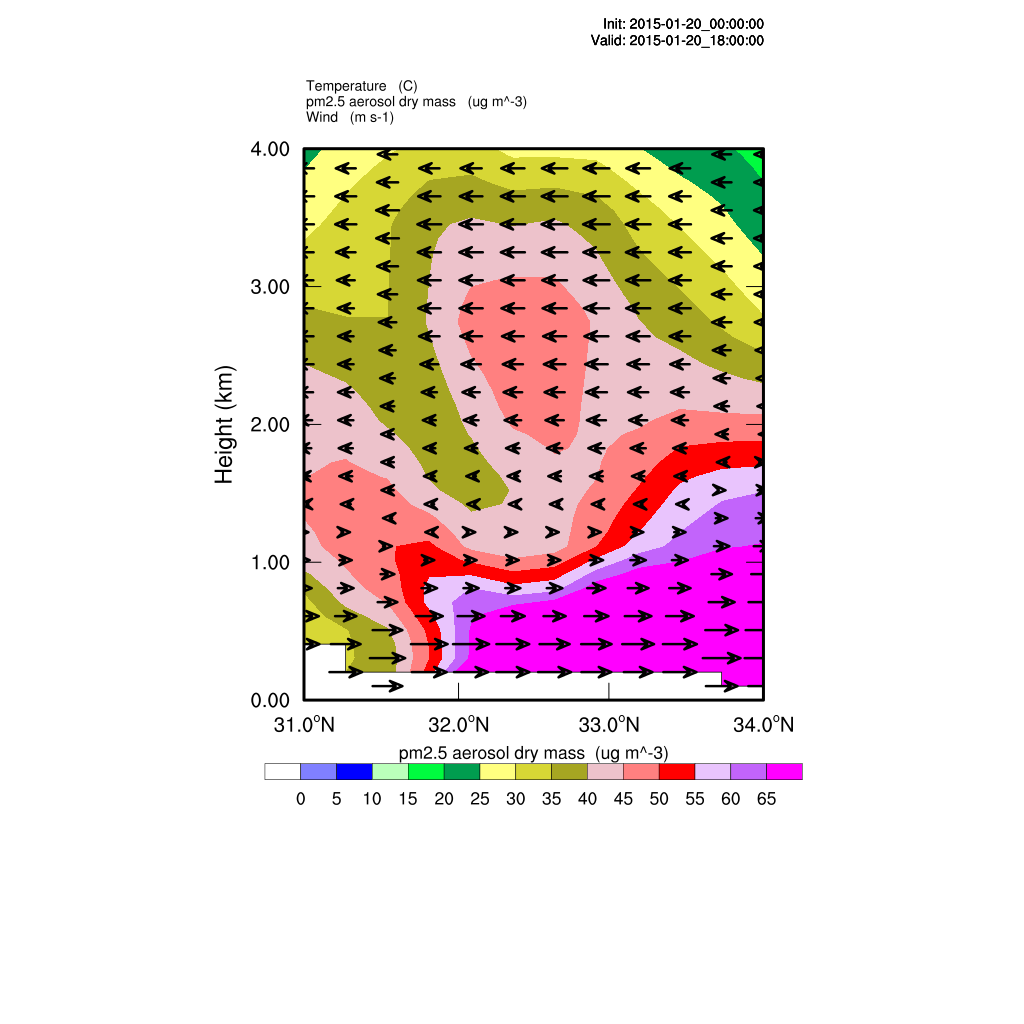
\includegraphics[width=\textwidth]{pm25_19}
		\caption{}
		\label{fig:pm25_19}
	\end{subfigure}%
	~% add desired spacing
	\\% line break
	\begin{subfigure}[b]{0.35\textwidth}
		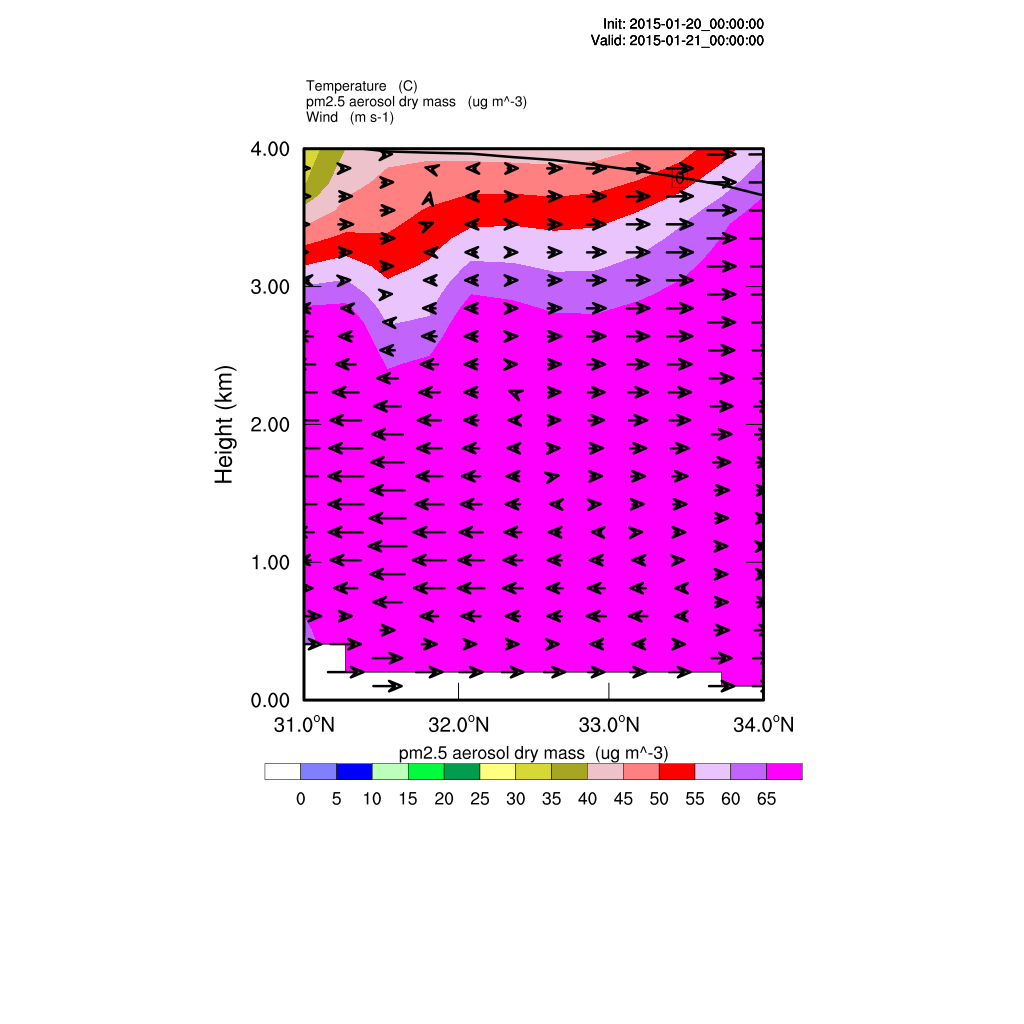
\includegraphics[width=\textwidth]{pm25_25}
		\caption{}
		\label{fig:pm25_25}
	\end{subfigure}%
	\begin{subfigure}[b]{0.35\textwidth}
		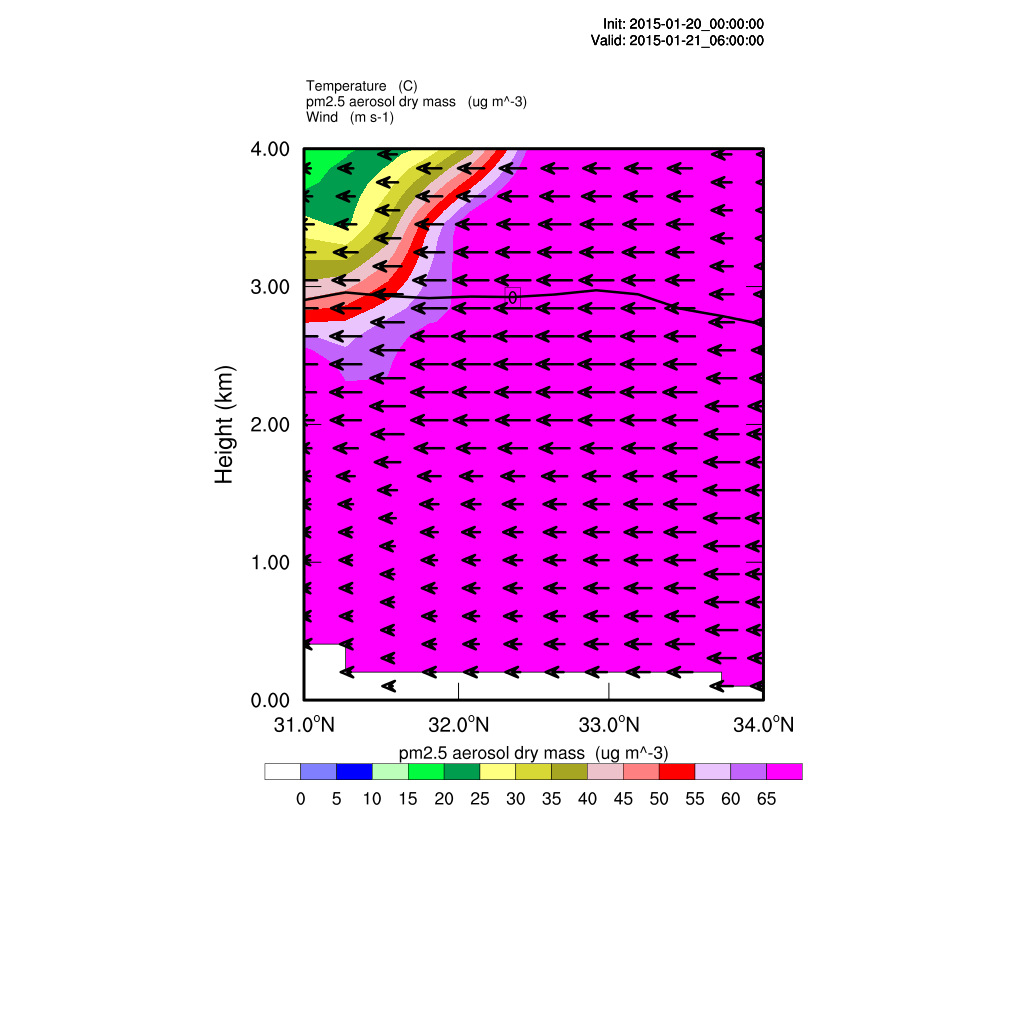
\includegraphics[width=\textwidth]{pm25_31}
		\caption{}
		\label{fig:pm25_31}
	\end{subfigure}%
	\begin{subfigure}[b]{0.35\textwidth}
		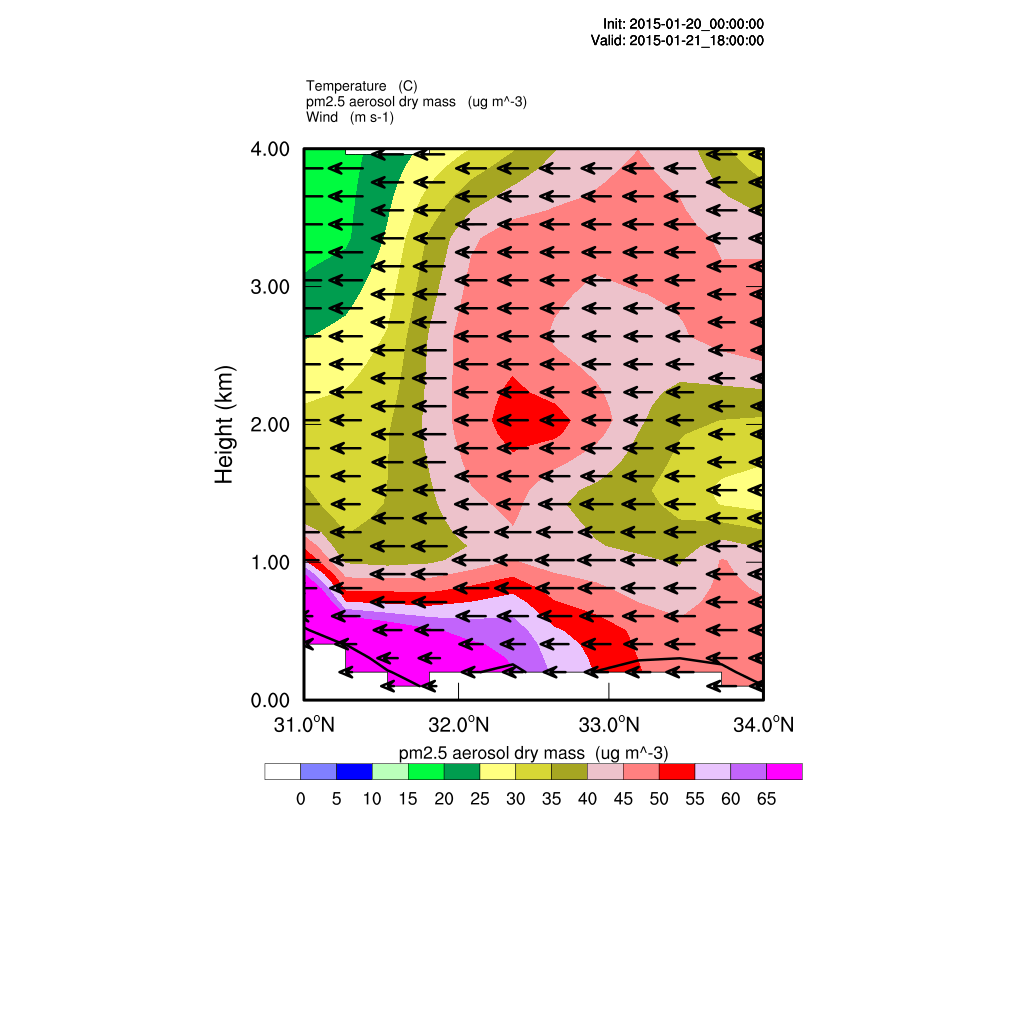
\includegraphics[width=\textwidth]{pm25_43}
		\caption{}
		\label{fig:pm25_43}
	\end{subfigure}%
	\bicaption{$PM_{2.5}$浓度剖面图 (a) 1月20日07时500,(b) 1月21日07时,(c) 1月21日07时,(d) 1月22日07时。}{Surface $PM_{2.5}$ concentration superimposed wind field map (a) 07 a.m. on 20 January, (b) 07 a.m. on 21 January, (c) 07 a.m. on 22 January, (d) 07 a.m. on 23 January.}
	\label{fig:oaspl}
\end{figure}


%---------------------------------------------------------------------------%
% main content
%-
%-> Appendix
%-
%\cleardoublepage%
%\appendix% initialize the environment
%\chapter{中国科学院大学学位论文撰写要求}

学位论文是研究生科研工作成果的集中体现,是评判学位申请者学术水平、授予其学位的主要依据,是科研领域重要的文献资料。根据《科学技术报告、学位论文和学术论文的编写格式》(GB/T 7713-1987)、《学位论文编写规则》(GB/T 7713.1-2006)和《文后参考文献著录规则》(GB7714—87)等国家有关标准,结合中国科学院大学(以下简称“国科大”)的实际情况,特制订本规定。

\section{论文无附录者无需附录部分}

\section{测试公式编号 \texorpdfstring{$\Lambda,\lambda,\theta,\bar{\Lambda},\sqrt{S_{NN}}$}{$\textLambda,\textlambda,\texttheta,\bar{\textLambda},\sqrt{S_{NN}}$}} \label{sec:testmath}

\begin{equation} \label{eq:appedns}
    \adddotsbeforeeqnnum%
    \begin{cases}
        \frac{\partial \rho}{\partial t} + \nabla\cdot(\rho\Vector{V}) = 0\\
        \frac{\partial (\rho\Vector{V})}{\partial t} + \nabla\cdot(\rho\Vector{V}\Vector{V}) = \nabla\cdot\Tensor{\sigma}\\
        \frac{\partial (\rho E)}{\partial t} + \nabla\cdot(\rho E\Vector{V}) = \nabla\cdot(k\nabla T) + \nabla\cdot(\Tensor{\sigma}\cdot\Vector{V})
    \end{cases}
\end{equation}
\begin{equation}
    \adddotsbeforeeqnnum%
    \frac{\partial }{\partial t}\int\limits_{\Omega} u \, \mathrm{d}\Omega + \int\limits_{S} \unitVector{n}\cdot(u\Vector{V}) \, \mathrm{d}S = \dot{\phi}
\end{equation}
\[
    \begin{split}
        \mathcal{L} \{f\}(s) &= \int _{0^{-}}^{\infty} f(t) e^{-st} \, \mathrm{d}t, \ 
        \mathscr{L} \{f\}(s) = \int _{0^{-}}^{\infty} f(t) e^{-st} \, \mathrm{d}t\\
        \mathcal{F} {\bigl (} f(x+x_{0}) {\bigr )} &= \mathcal{F} {\bigl (} f(x) {\bigr )} e^{2\pi i\xi x_{0}}, \ 
        \mathscr{F} {\bigl (} f(x+x_{0}) {\bigr )} = \mathscr{F} {\bigl (} f(x) {\bigr )} e^{2\pi i\xi x_{0}}
    \end{split}
\]

mathtext: $A,F,L,2,3,5,\sigma$, mathnormal: $A,F,L,2,3,5,\sigma$, mathrm: $\mathrm{A,F,L,2,3,5,\sigma}$.

mathbf: $\mathbf{A,F,L,2,3,5,\sigma}$, mathit: $\mathit{A,F,L,2,3,5,\sigma}$, mathsf: $\mathsf{A,F,L,2,3,5,\sigma}$.

mathtt: $\mathtt{A,F,L,2,3,5,\sigma}$, mathfrak: $\mathfrak{A,F,L,2,3,5,\sigma}$, mathbb: $\mathbb{A,F,L,2,3,5,\sigma}$.

mathcal: $\mathcal{A,F,L,2,3,5,\sigma}$, mathscr: $\mathscr{A,F,L,2,3,5,\sigma}$, boldsymbol: $\boldsymbol{A,F,L,2,3,5,\sigma}$.

vector: $\Vector{\sigma, T, a, F, n}$, unitvector: $\unitVector{\sigma, T, a, F, n}$

matrix: $\Matrix{\sigma, T, a, F, n}$, unitmatrix: $\unitMatrix{\sigma, T, a, F, n}$

tensor: $\Tensor{\sigma, T, a, F, n}$, unittensor: $\unitTensor{\sigma, T, a, F, n}$ 

\section{测试生僻字}

霜蟾盥薇曜灵霜颸妙鬘虚霩淩澌菀枯菡萏泬寥窅冥毰毸濩落霅霅便嬛岧峣瀺灂姽婳愔嫕飒纚棽俪緸冤莩甲摛藻卮言倥侗椒觞期颐夜阑彬蔚倥偬澄廓簪缨陟遐迤逦缥缃鹣鲽憯懔闺闼璀错媕婀噌吰澒洞阛闠覼缕玓瓑逡巡諓諓琭琭瀌瀌踽踽叆叇氤氲瓠犀流眄蹀躞赟嬛茕頔璎珞螓首蘅皋惏悷缱绻昶皴皱颟顸愀然菡萏卑陬纯懿犇麤掱暒 墌墍墎墏墐墒墒墓墔墕墖墘墖墚墛坠墝增墠墡墢墣墤墥墦墧墨墩墪樽墬墭堕墯墰墱墲坟墴墵垯墷墸墹墺墙墼墽垦墿壀壁壂壃壄壅壆坛壈壉壊垱壌壍埙壏壐壑壒压壔壕壖壗垒圹垆壛壜壝垄壠壡坜壣壤壥壦壧壨坝塆圭嫶嫷嫸嫹嫺娴嫼嫽嫾婳妫嬁嬂嬃嬄嬅嬆嬇娆嬉嬊娇嬍嬎嬏嬐嬑嬒嬓嬔嬕嬖嬗嬘嫱嬚嬛嬜嬞嬟嬠嫒嬢嬣嬥嬦嬧嬨嬩嫔嬫嬬奶嬬嬮嬯婴嬱嬲嬳嬴嬵嬶嬷婶嬹嬺嬻嬼嬽嬾嬿孀孁孂娘孄孅孆孇孆孈孉孊娈孋孊孍孎孏嫫婿媚嵭嵮嵯嵰嵱嵲嵳嵴嵵嵶嵷嵸嵹嵺嵻嵼嵽嵾嵿嶀嵝嶂嶃崭嶅嶆岖嶈嶉嶊嶋嶌嶍嶎嶏嶐嶑嶒嶓嵚嶕嶖嶘嶙嶚嶛嶜嶝嶞嶟峤嶡峣嶣嶤嶥嶦峄峃嶩嶪嶫嶬嶭崄嶯嶰嶱嶲嶳岙嶵嶶嶷嵘嶹岭嶻屿岳帋巀巁巂巃巄巅巆巇巈巉巊岿巌巍巎巏巐巑峦巓巅巕岩巗巘巙巚帠帡帢帣帤帨帩帪帬帯帰帱帲帴帵帷帹帺帻帼帽帾帿幁幂帏幄幅幆幇幈幉幊幋幌幍幎幏幐幑幒幓幖幙幚幛幜幝幞帜幠幡幢幤幥幦幧幨幩幪幭幮幯幰幱庍庎庑庖庘庛庝庠庡庢庣庤庥庨庩庪庬庮庯庰庱庲庳庴庵庹庺庻庼庽庿廀厕廃厩廅廆廇廋廌廍庼廏廐廑廒廔廕廖廗廘廙廛廜廞庑廤廥廦廧廨廭廮廯廰痈廲廵廸廹廻廼廽廿弁弅弆弇弉弖弙弚弜弝弞弡弢弣弤弨弩弪弫弬弭弮弰弲弪弴弶弸弻弼弽弿彖彗彘彚彛彜彝彞彟彴彵彶彷彸役彺彻彽彾佛徂徃徆徇徉后徍徎徏径徒従徔徕徖徙徚徛徜徝从徟徕御徢徣徤徥徦徧徨复循徫旁徭微徯徰徱徲徳徴徵徶德徸彻徺忁忂惔愔忇忈忉忔忕忖忚忛応忝忞忟忪挣挦挧挨挩挪挫挬挭挮挰掇授掉掊掋掍掎掐掑排掓掔掕挜掚挂掜掝掞掟掠采探掣掤掦措掫掬掭掮掯掰掱掲掳掴掵掶掸掹掺掻掼掽掾掿拣揁揂揃揅揄揆揇揈揉揊揋揌揍揎揑揓揔揕揖揗揘揙揤揥揦揧揨揫捂揰揱揲揳援揵揶揷揸揻揼揾揿搀搁搂搃搄搅搇搈搉搊搋搌搎搏搐搑搒摓摔摕摖摗摙摚摛掼摝摞摠摡斫斩斮斱斲斳斴斵斶斸旪旫旮旯晒晓晔晕晖晗晘晙晛晜晞晟晠晡晰晣晤晥晦晧晪晫晬晭晰晱晲晳晴晵晷晸晹晻晼晽晾晿暀暁暂暃暄暅暆暇晕晖暊暋暌暍暎暏暐暑暒暓暔暕暖暗旸暙暚暛暜暝暞暟暠暡暣暤暥暦暧暨暩暪暬暭暮暯暰昵暲暳暴暵

% appendix content
%-
%-> Backmatter: bibliography, glossary, index
%-
\backmatter% initialize the environment
\intotoc*{\cleardoublepage}{\bibname}% add link to toc
\bibliography{Biblio/ref}% bibliography
%---------------------------------------------------------------------------%
%->> Backmatter
%---------------------------------------------------------------------------%
\chapter[致谢]{致\quad 谢}\chaptermark{致\quad 谢}% syntax: \chapter[目录]{标题}\chaptermark{页眉}
\thispagestyle{noheaderstyle}% 如果需要移除当前页的页眉
%\pagestyle{noheaderstyle}% 如果需要移除整章的页眉

感激casthesis作者吴凌云学长,gbt7714-bibtex-style
开发者zepinglee,和ctex众多开发者们。若没有他们的辛勤付出和非凡工作,\LaTeX{}菜鸟的我是无法完成此国科大学位论文\LaTeX{}模板ucasthesis的。在\LaTeX{}中的一点一滴的成长源于开源社区的众多优秀资料和教程,在此对所有\LaTeX{}社区的贡献者表示感谢!

ucasthesis国科大学位论文\LaTeX{}模板的最终成型离不开以霍明虹老师和丁云云老师为代表的国科大学位办公室老师们制定的官方指导文件和众多ucasthesis用户的热心测试和耐心反馈,在此对他们的认真付出表示感谢。特别对国科大的赵永明同学的众多有效反馈意见和建议表示感谢,对国科大本科部的陆晴老师和本科部学位办的丁云云老师的细致审核和建议表示感谢。谢谢大家的共同努力和支持,让ucasthesis为国科大学子使用\LaTeX{}撰写学位论文提供便利和高效这一目标成为可能。

\cleardoublepage[plain]% 让文档总是结束于偶数页,可根据需要设定页眉页脚样式,如 [noheaderstyle]
%---------------------------------------------------------------------------%
% other information
\end{document}
%---------------------------------------------------------------------------%

